% ============ MAIN.TEX ============
\documentclass[12pt]{article}

% Gọi file cấu hình
\input{preamble.tex}

% ============ DOCUMENT ============
\begin{document}

\pagenumbering{roman}

% Gọi trang bìa
\input{sections/00_trang_bia.tex}

\tableofcontents
\pagebreak
\listoftables
\pagebreak
\listoffigures
\pagebreak

\pagenumbering{arabic}
\setcounter{page}{1}

% ============ NỘI DUNG ============
% ===========================================================================
% File: sections/01_introduction.tex
% Phần 1: Giới thiệu
% Thuộc tutorial: The Science of Benchmarking — What's Measured, What's Missing, What's Next
% Thành viên 1: Nền tảng benchmarking và câu hỏi "Benchmark đo cái gì?"
% ===========================================================================

\section{Giới thiệu}
\label{sec:introduction}

Benchmark đóng vai trò trung tâm trong quá trình phát triển và đánh giá các hệ thống trí tuệ nhân tạo (AI) và học máy (ML). Trong nghiên cứu, benchmark cung cấp khung tham chiếu chung để so sánh hiệu năng giữa các mô hình, theo dõi tiến bộ theo thời gian và xác định hướng đi cho các nỗ lực nghiên cứu tiếp theo. Benchmark cũng là công cụ không thể thiếu trong quy trình công bố kết quả khoa học: một mô hình được coi là ``state-of-the-art'' (SOTA) khi đạt điểm số cao nhất trên một hoặc nhiều benchmark được cộng đồng thừa nhận~\cite{everything_benchmark}. Trong bối cảnh các mô hình ngôn ngữ lớn (Large Language Models -- LLM) phát triển nhanh chóng, benchmark trở thành yếu tố then chốt để đánh giá năng lực, phát hiện rủi ro an toàn và hướng dẫn triển khai~\cite{measuring_what_matters}.

Tuy nhiên, benchmark thường được sử dụng vượt xa phạm vi thiết kế ban đầu. Điểm số trên một benchmark cụ thể dễ dàng bị diễn giải như bằng chứng cho tiến bộ AI nói chung, thậm chí được xem như thước đo cho ``trí tuệ'' hay ``năng lực tổng quát'' của hệ thống. Raji và cộng sự~\cite{everything_benchmark} đã chỉ ra rằng nhiều benchmark phổ biến, dù chỉ đo hiệu năng trên một tập hữu hạn các tác vụ cụ thể, lại được cộng đồng nâng lên thành đại diện cho năng lực chung (\textit{general capabilities}). Điều này tương tự như việc một bảo tàng tuyên bố chứa ``mọi thứ trên thế giới'' nhưng thực tế chỉ trưng bày một số phòng với các vật phẩm được chọn tùy tiện. Bean và cộng sự~\cite{measuring_what_matters} bổ sung rằng giá trị thực sự của một benchmark phụ thuộc vào việc nó có phải là một \textit{proxy} tốt cho hiện tượng (phenomenon) mà nó định đo hay không --- một thuộc tính được gọi là \textit{construct validity}.

Tutorial này --- \textit{The Science of Benchmarking: What's Measured, What's Missing, What's Next} --- nhằm phân tích một cách có hệ thống khoa học đằng sau benchmarking trong AI/ML. Luận điểm trung tâm của phần này là:

\begin{summarybox}
\textit{Benchmark không phải là thước đo tuyệt đối của trí tuệ hay năng lực tổng quát; benchmark là một công cụ đo lường có phạm vi, giả định, thiết kế và giới hạn diễn giải.}
\end{summarybox}

Từ luận điểm này, phần nền tảng của báo cáo sẽ đặt ra và trả lời câu hỏi trung tâm:

\begin{summarybox}
\textit{Benchmark thực sự đang đo cái gì?}
\end{summarybox}

Để trả lời câu hỏi trên, các phần tiếp theo sẽ trình bày bối cảnh và động lực của benchmarking trong AI (Phần~\ref{sec:background}), các khái niệm nền tảng về benchmark và đo lường (Phần~\ref{sec:foundations}), vai trò của construct validity trong benchmark LLM (Phần~\ref{sec:construct_validity}), và phân tích cụ thể về những gì benchmark hiện nay thực sự đang đo (Phần~\ref{sec:whats_measured}).
% ===========================================================================
% File: sections/02_background.tex
% Phần 2: Bối cảnh và động lực của AI benchmarking
% Thuộc tutorial: The Science of Benchmarking — What's Measured, What's Missing, What's Next
% Thành viên 1: Nền tảng benchmarking và câu hỏi "Benchmark đo cái gì?"
% ===========================================================================

\section{Bối cảnh và động lực của AI benchmarking}
\label{sec:background}

\subsection{Vì sao AI/ML cần benchmark?}

Benchmark ra đời từ nhu cầu thực tiễn: cung cấp một khung tham chiếu chung để so sánh hiệu năng giữa các phương pháp khác nhau trên cùng một tác vụ. Trước khi benchmark được sử dụng rộng rãi trong ML, việc đánh giá thuật toán thường thiếu tính nhất quán --- mỗi nhóm nghiên cứu sử dụng dữ liệu riêng, protocol riêng và metric riêng, khiến việc so sánh kết quả trở nên khó khăn, thậm chí vô nghĩa~\cite{everything_benchmark}.

Mô hình Common Task Framework (CTF), được phát triển từ thập niên 1980 dưới sự dẫn dắt của Fred Jelinek (IBM) và Charles Wayne (DARPA), đã thiết lập nền tảng cho benchmarking hiện đại. CTF bao gồm ba thành phần chính: (a) tập dữ liệu huấn luyện công khai với nhãn, (b) một nhóm người tham gia cùng giải quyết tác vụ chung, và (c) một trọng tài chấm điểm để đánh giá kết quả~\cite{everything_benchmark}. Với CTF, thay vì chỉ cập nhật kết quả thực nghiệm ``hai lần mỗi năm'', các nhà nghiên cứu có thể đánh giá thí nghiệm hàng giờ và theo dõi tiến bộ liên tục.

Trong bối cảnh hiện đại, benchmark phục vụ nhiều mục đích quan trọng:

\begin{itemize}
    \item \textbf{Chuẩn hóa so sánh}: Benchmark cung cấp tập dữ liệu, tác vụ và metric thống nhất, cho phép cộng đồng so sánh công bằng giữa các mô hình.
    \item \textbf{Theo dõi tiến bộ}: Bảng xếp hạng (leaderboard) dựa trên benchmark giúp theo dõi sự cải thiện hiệu năng theo thời gian.
    \item \textbf{Lựa chọn mô hình}: Kết quả benchmark hỗ trợ quyết định lựa chọn mô hình cho các ứng dụng cụ thể.
    \item \textbf{Định hướng nghiên cứu}: Benchmark ảnh hưởng mạnh đến hướng phát triển thuật toán và phân bổ nguồn lực nghiên cứu của cả lĩnh vực~\cite{everything_benchmark}.
\end{itemize}

\subsection{Mặt trái của benchmarking}

Mặc dù có vai trò không thể phủ nhận, benchmarking tiềm ẩn nhiều rủi ro nghiêm trọng khi bị sử dụng hoặc diễn giải không đúng cách.

\subsubsection{Leaderboard chasing và tối ưu hóa quá mức}

Việc chạy đua đạt điểm số ``state-of-the-art'' (SOTA) trên benchmark --- hay \textit{leaderboard chasing} --- là một hiện tượng phổ biến trong cộng đồng ML. Saitta đã từ năm 1995 chỉ trích rằng benchmark chasing ``cho phép các nhà nghiên cứu công bố những bài báo nhàm chán, đề xuất các biến thể nhỏ của thuật toán học có giám sát hiện có và báo cáo những cải thiện hiệu năng nhỏ nhưng có ý nghĩa thống kê''; Thomas và Uminsky còn xem việc chạy đua theo metric là một vấn đề đạo đức, cảnh báo rằng ``việc nhấn mạnh quá mức vào metric dẫn đến thao túng, gaming, tập trung thiển cận vào mục tiêu ngắn hạn và các hậu quả tiêu cực không mong đợi khác''~\cite{everything_benchmark}.

Hệ quả của leaderboard chasing là cộng đồng có xu hướng tối ưu hóa quá mức (\textit{overfitting}) trên một benchmark cụ thể, thay vì cải thiện năng lực thực sự của mô hình. Khi cả lĩnh vực tập trung vào một số ít benchmark, các kỹ thuật mới được phát triển sẽ đặc biệt phù hợp với các tác vụ đó, dẫn đến hiện tượng overfitting ở cấp độ cộng đồng~\cite{measuring_what_matters}.

\subsubsection{Diễn giải sai điểm benchmark}

Một rủi ro nghiêm trọng khác là việc diễn giải điểm benchmark vượt quá phạm vi thiết kế. Raji và cộng sự~\cite{everything_benchmark} chỉ ra rằng các benchmark như ImageNet hay GLUE, dù chỉ đo hiệu năng trên các tác vụ hẹp và cụ thể, lại thường được trình bày và chấp nhận như thước đo cho năng lực tổng quát, và dẫn ra ví dụ Microsoft năm 2021 tuyên bố rằng ``DeBERTa vượt qua hiệu năng con người trên SuperGLUE đánh dấu một cột mốc quan trọng hướng tới AI tổng quát''. Tuy nhiên, hiệu năng cao trên SuperGLUE --- một tập hợp các tác vụ phân loại câu và cặp câu trong tiếng Anh --- không tương đương với ``hiểu ngôn ngữ'' hay ``trí tuệ tổng quát''.

Wagstaff~\cite{everything_benchmark} cũng cảnh báo rằng cùng một mức độ chính xác (ví dụ 80\%) có ý nghĩa hoàn toàn khác nhau trong các bối cảnh khác nhau: 80\% chính xác trong phân loại hoa iris có thể chấp nhận được, nhưng 80\% trong phân loại nấm ăn được hay nấm độc là hoàn toàn không đủ, và giả định về tính so sánh xuyên miền (cross-domain comparability) khi sử dụng cùng loại metric là một ``ảo ảnh''.

\subsubsection{Benchmark như đại diện quá rộng cho năng lực AI}

Benchmark ban đầu được thiết kế để đánh giá hiệu năng trên các tác vụ cụ thể, ứng dụng thực tiễn --- ví dụ nhận dạng giọng nói (ASR) hay dịch máy (MT)~\cite{everything_benchmark}. Tuy nhiên, xu hướng gần đây đã mở rộng không phù hợp mô hình CTF sang việc đo ``hiệu năng nói chung'' (\textit{performance in the abstract}), tách rời khỏi mục tiêu thực tế hay ngữ cảnh ứng dụng; Raji và cộng sự lập luận rằng mục tiêu đo năng lực tổng quát (general-purpose capabilities) không thể được hiện thực hóa đầy đủ trong các benchmark dựa trên dữ liệu, bởi dữ liệu luôn có phạm vi hữu hạn, mang tính chủ quan và bị giới hạn bởi bối cảnh~\cite{everything_benchmark}.

\subsection{Goodhart's Law và benchmark}

Mối quan hệ giữa benchmark và tối ưu hóa có thể được hiểu rõ hơn qua lăng kính của Goodhart's Law:

\begin{quote}
\textit{Khi một thước đo trở thành mục tiêu tối ưu hóa, nó có thể mất dần giá trị như một thước đo đáng tin cậy.}
\end{quote}

Trong bối cảnh AI benchmarking, hiện tượng này biểu hiện ở nhiều cấp độ. Ở cấp độ mô hình, khi một benchmark được sử dụng rộng rãi, nỗ lực liên tục cải thiện trên benchmark đó dẫn đến các kỹ thuật mới được phát triển đặc biệt phù hợp với tác vụ cụ thể đó, gây ra hiện tượng overfitting tương tự như việc sử dụng lặp lại tập validation~\cite{measuring_what_matters}. Ở cấp độ cộng đồng, benchmark ảnh hưởng đến bản chất của các phương pháp thuật toán được theo đuổi: trong thập niên 1960, cờ vua khiến cộng đồng AI tập trung quá mức vào deep-tree searching và thuật toán minimax; tương tự, ImageNet đã định hình cuộc cách mạng deep learning và GLUE đã trở thành nền tảng chứng minh cho BERT~\cite{everything_benchmark}.

\subsection{Data contamination}

\textit{Data contamination} --- hiện tượng dữ liệu đánh giá xuất hiện trong dữ liệu huấn luyện hoặc quá trình tinh chỉnh mô hình --- là một mối đe dọa nghiêm trọng đối với tính hợp lệ của kết quả benchmark. Bean và cộng sự~\cite{measuring_what_matters} nhấn mạnh rằng contamination có thể xảy ra ngay cả khi các nhà phát triển mô hình hành động thiện chí, bởi các tập dữ liệu benchmark công khai có khả năng cao đã xuất hiện trong các kho dữ liệu huấn luyện quy mô lớn; với các benchmark phổ biến như GSM8K, bằng chứng cho thấy contamination có thể đã góp phần làm tăng điểm số theo thời gian.

\subsection{Tóm tắt: Benchmark vừa cần thiết, vừa cần thận trọng}

Benchmark là công cụ thiết yếu trong nghiên cứu AI/ML, cho phép chuẩn hóa đánh giá, theo dõi tiến bộ và so sánh phương pháp. Tuy nhiên, giá trị của benchmark phụ thuộc vào cách nó được thiết kế, sử dụng và diễn giải. Khi benchmark bị đối xử như thước đo toàn diện cho ``trí tuệ'' hay ``tiến bộ AI nói chung'', nó trở thành nguồn gây hiểu lầm. Như Raji và cộng sự~\cite{everything_benchmark} kết luận, vấn đề không nằm ở bản thân benchmark, mà ở cách cộng đồng định khung và nâng tầm benchmark vượt quá phạm vi thiết kế ban đầu. Các phần tiếp theo sẽ đi sâu vào khung khái niệm cần thiết để hiểu rõ benchmark đo cái gì và không đo cái gì.
% ===========================================================================
% File: sections/03_foundations.tex
% Phần 3: Kiến thức nền về benchmark và đo lường
% Thuộc tutorial: The Science of Benchmarking — What's Measured, What's Missing, What's Next
% Thành viên 1: Nền tảng benchmarking và câu hỏi "Benchmark đo cái gì?"
% ===========================================================================

\section{Kiến thức nền về benchmark và đo lường}
\label{sec:foundations}

Phần này trình bày các khái niệm nền tảng cần thiết để phân tích benchmark một cách có hệ thống. Các khái niệm được giải thích trong bối cảnh đánh giá AI/ML và benchmark LLM. Trọng tâm của phần này là làm rõ benchmark không chỉ là một tập dữ liệu, mà là một cấu hình đo lường gồm tác vụ, dữ liệu, metric, quy trình đánh giá, giả định diễn giải và các điều kiện ảnh hưởng đến ý nghĩa của điểm số.

\subsection{Benchmark và dataset: Sự khác biệt cơ bản}
\label{sec:benchmark_vs_dataset}

Trong thực tiễn, thuật ngữ ``benchmark'' và ``dataset'' thường được sử dụng thay thế cho nhau. Tuy nhiên, hai khái niệm này có phạm vi và bản chất khác nhau.

\textbf{Dataset} là một tập hợp dữ liệu --- bao gồm các mẫu đầu vào, nhãn hoặc đầu ra mong đợi --- được thu thập và tổ chức cho một mục đích cụ thể. Dataset tự nó chỉ là nguyên liệu; nó không định nghĩa cách đánh giá, không chỉ định metric, và không đi kèm đầy đủ các giả định về năng lực nào đang được đo.

\textbf{Benchmark} là một cấu hình đánh giá hoàn chỉnh, bao gồm nhiều thành phần được thiết kế có chủ đích để đo lường hiệu năng của hệ thống trên một tác vụ hoặc năng lực cụ thể. Raji và cộng sự~\cite{everything_benchmark} định nghĩa benchmark là ``một sự kết hợp cụ thể của dataset (ít nhất là dữ liệu kiểm tra, đôi khi cả dữ liệu huấn luyện) và metric, được khái niệm hóa như đại diện cho một hoặc nhiều tác vụ hoặc tập hợp năng lực cụ thể, được cộng đồng nghiên cứu chấp nhận như khung tham chiếu chung để so sánh phương pháp''. Bean và cộng sự~\cite{measuring_what_matters} bổ sung rằng benchmark bao gồm \textit{task} (tác vụ) và \textit{metric} (thước đo) được sử dụng cùng nhau để đại diện cho một \textit{phenomenon} (hiện tượng) cần đo.

Nói cách khác, dataset là một thành phần của benchmark, nhưng không tương đương với benchmark. Một benchmark chỉ hình thành đầy đủ khi dữ liệu được đặt trong một cấu hình đánh giá có tác vụ, metric, protocol và cách diễn giải điểm số.

\subsection{Các thành phần cốt lõi của benchmark}
\label{sec:benchmark_components}

Một benchmark hoàn chỉnh thường bao gồm các thành phần sau:

\begin{itemize}
    \item \textbf{Task} (tác vụ): Đặc tả cụ thể của vấn đề cần giải quyết, được hiện thực hóa trong dataset~\cite{everything_benchmark}.
    \item \textbf{Data} (dữ liệu): Tập hợp các mẫu kiểm tra, đôi khi bao gồm cả dữ liệu huấn luyện.
    \item \textbf{Metric} (thước đo): Cách tổng hợp hiệu năng hệ thống thành một con số hoặc điểm số~\cite{everything_benchmark}.
    \item \textbf{Protocol} (quy trình đánh giá): Các quy tắc về cách thức tiến hành đánh giá.
    \item \textbf{Assumptions} (giả định): Các giả định ngầm về năng lực nào đang được đo và bối cảnh áp dụng.
    \item \textbf{Interpretation} (diễn giải): Cách thức điểm số được hiểu và sử dụng~\cite{measuring_what_matters}.
\end{itemize}

Các thành phần này cho thấy benchmark là một hệ thống đo lường. Do đó, khi phân tích một benchmark, không thể chỉ xem xét dữ liệu kiểm tra hoặc điểm số cuối cùng, mà cần xem xét toàn bộ cấu hình đánh giá và các giả định đứng sau nó.

% Bảng tổng hợp các khái niệm nền tảng
% Yêu cầu package: longtable, booktabs, needspace
\Needspace{10\baselineskip}

\small
\setlength{\tabcolsep}{6pt}
\renewcommand{\arraystretch}{1.2}

\begin{longtable}{p{4cm} p{12cm}}
\caption{Tổng hợp các khái niệm nền tảng trong benchmark và đo lường AI/ML.}
\label{tab:concepts} \\

\toprule
\textbf{Khái niệm} & \textbf{Giải thích} \\
\midrule
\endfirsthead

\toprule
\textbf{Khái niệm} & \textbf{Giải thích} \\
\midrule
\endhead

Benchmark &
Cấu hình đánh giá hoàn chỉnh gồm dataset, task, metric, protocol và giả định diễn giải; được cộng đồng sử dụng để so sánh phương pháp~\cite{everything_benchmark, measuring_what_matters}. \\
\addlinespace

Dataset &
Tập hợp dữ liệu gồm đầu vào, nhãn hoặc đầu ra mong đợi; là thành phần của benchmark nhưng không tương đương benchmark. \\
\addlinespace

Task &
Đặc tả tác vụ mà hệ thống cần thực hiện; task là cầu nối giữa dữ liệu cụ thể và năng lực hoặc hiện tượng mà benchmark muốn đại diện~\cite{everything_benchmark, measuring_what_matters}. \\
\addlinespace

Metric &
Cách thức tổng hợp hiệu năng hệ thống trên tập mẫu thành một con số tóm tắt; ví dụ: accuracy, F1-score, exact match~\cite{everything_benchmark}. \\
\addlinespace

Evaluation protocol &
Tập hợp các quy tắc và điều kiện tiến hành đánh giá, bao gồm định dạng đầu ra, số lượng lần chạy, cách xử lý câu trả lời, và các ràng buộc kỹ thuật khác. \\
\addlinespace

Construct &
Khái niệm trừu tượng hoặc năng lực mà benchmark định đo; ví dụ: \textit{reasoning}, \textit{safety}, \textit{robustness}~\cite{measuring_what_matters}. \\
\addlinespace

Construct validity &
Mức độ mà điểm benchmark cung cấp bằng chứng hợp lệ cho các nhận định về construct mục tiêu~\cite{measuring_what_matters, everything_benchmark}. \\
\addlinespace

Validity &
Tính chất phản ánh liệu phép đo có thực sự đo đúng điều cần đo hay không; bao gồm face validity, content validity, predictive validity, convergent validity và discriminant validity~\cite{measuring_what_matters}. \\
\addlinespace

Reliability &
Tính chất phản ánh liệu kết quả đo có ổn định và lặp lại được hay không khi thực hiện trong các điều kiện tương tự~\cite{everything_benchmark}. \\
\addlinespace

Reproducibility &
Khả năng tái tạo kết quả đánh giá khi sử dụng cùng dữ liệu, mô hình và protocol bởi các nhóm nghiên cứu khác nhau. \\
\addlinespace

Statistical significance &
Đánh giá xem sự khác biệt trong điểm số giữa các mô hình có đáng tin cậy, không chỉ là kết quả của nhiễu ngẫu nhiên, hay không~\cite{measuring_what_matters}. \\
\addlinespace

Data contamination &
Hiện tượng dữ liệu đánh giá xuất hiện trong dữ liệu huấn luyện hoặc quá trình tinh chỉnh mô hình, làm suy giảm tính hợp lệ của kết quả~\cite{measuring_what_matters}. \\
\addlinespace

Benchmark overfitting &
Hiện tượng mô hình hoặc cộng đồng tối ưu hóa quá mức trên một benchmark cụ thể, dẫn đến điểm số cao nhưng không phản ánh đầy đủ năng lực ngoài benchmark~\cite{everything_benchmark, measuring_what_matters}. \\
\addlinespace

Goodhart's Law &
Khi một thước đo trở thành mục tiêu tối ưu hóa, nó mất dần giá trị như thước đo đáng tin cậy. \\
\bottomrule
\end{longtable}

\normalsize

\subsection{Metric và evaluation protocol}
\label{sec:metric_protocol}

Metric và evaluation protocol là hai thành phần vận hành trực tiếp của benchmark. Metric xác định cách lượng hóa kết quả, trong khi protocol xác định điều kiện mà kết quả đó được tạo ra. Vì vậy, cùng một dataset có thể dẫn đến các kết luận khác nhau nếu metric hoặc protocol thay đổi.

\subsubsection{Metric: Cách lượng hóa, không phải bảo đảm}
\label{sec:metric}

Metric là thành phần thiết yếu của benchmark, cung cấp cách thức lượng hóa hiệu năng hệ thống. Raji và cộng sự~\cite{everything_benchmark} định nghĩa metric là ``cách tổng hợp hiệu năng hệ thống trên một tập hoặc các tập tác vụ thành một con số hoặc điểm số đơn lẻ''. Trong khảo sát 445 benchmark LLM, Bean và cộng sự~\cite{measuring_what_matters} phát hiện rằng metric phổ biến nhất là exact match, được sử dụng ít nhất một phần bởi 81,3\% benchmark, tiếp theo là soft match với 20,9\%, LLM-as-a-judge với 17,1\% và đánh giá bởi con người với 13,0\%.

Tuy nhiên, metric chỉ là cách lượng hóa kết quả; nó không tự động bảo đảm rằng benchmark đo đúng năng lực cần đo. Wagstaff~\cite{everything_benchmark} cảnh báo rằng việc sử dụng cùng loại metric, ví dụ accuracy, trên các tác vụ khác nhau tạo ra ``ảo ảnh về tính so sánh xuyên miền'', trong khi thực tế ý nghĩa của cùng mức accuracy có thể khác nhau giữa các bối cảnh. Ngoài ra, chỉ 16,0\% benchmark trong khảo sát sử dụng các phương pháp thống kê như uncertainty estimates hoặc statistical tests để so sánh kết quả giữa các mô hình~\cite{measuring_what_matters}.

Do đó, metric cần được hiểu như một phép tóm tắt hiệu năng có điều kiện, không phải một bảo đảm tuyệt đối về năng lực của hệ thống.

\subsubsection{Evaluation protocol và ảnh hưởng đến ý nghĩa điểm số}
\label{sec:protocol}

Evaluation protocol bao gồm cách thức trình bày tác vụ, định dạng đầu ra yêu cầu, số lượng lần chạy, cách xử lý kết quả và các ràng buộc kỹ thuật khác. Protocol có ảnh hưởng trực tiếp đến ý nghĩa điểm số vì nó xác định môi trường mà mô hình được đánh giá.

Bean và cộng sự~\cite{measuring_what_matters} chỉ ra rằng 21,1\% benchmark yêu cầu định dạng đầu ra cụ thể, tức structured output. Bản thân việc tuân thủ định dạng này đã có thể là một thử thách đối với mô hình, tách biệt khỏi năng lực mà benchmark định đo. Ví dụ, nếu một benchmark về reasoning yêu cầu đầu ra JSON, điểm số thấp có thể phản ánh khó khăn trong việc tạo JSON hơn là thiếu năng lực reasoning. Tương tự, các hướng dẫn phức tạp có thể làm giảm không cân xứng hiệu năng của các mô hình yếu hơn.

Vì vậy, khi diễn giải điểm benchmark, cần xem xét liệu điểm số phản ánh năng lực mục tiêu hay phản ánh các yêu cầu phụ do protocol tạo ra.

\subsection{Construct, validity và reliability}
\label{sec:construct_validity_reliability}

Một benchmark không chỉ tạo ra điểm số, mà còn tạo ra cơ sở để đưa ra nhận định về năng lực của hệ thống. Vì vậy, câu hỏi quan trọng không chỉ là ``mô hình đạt bao nhiêu điểm'', mà là ``điểm số đó có hỗ trợ hợp lệ cho nhận định nào về mô hình''.

\subsubsection{Construct và construct validity}
\label{sec:construct_validity}

\textbf{Construct} là khái niệm trừu tượng hoặc năng lực mà benchmark định đo, chẳng hạn như \textit{reasoning}, \textit{safety}, \textit{robustness}, \textit{factuality} hoặc \textit{general language understanding}~\cite{measuring_what_matters}. Trong benchmark AI/ML, construct thường không thể đo trực tiếp. Thay vào đó, benchmark sử dụng các task, dataset và metric cụ thể để đại diện cho construct đó.

\textbf{Construct validity} là mức độ mà điểm benchmark cung cấp bằng chứng hợp lệ cho các nhận định về construct mục tiêu~\cite{measuring_what_matters, everything_benchmark}. Nếu một benchmark được tuyên bố là đo reasoning, nhưng các câu hỏi có thể được giải bằng ghi nhớ mẫu, heuristic bề mặt hoặc dữ liệu đã bị contamination, thì construct validity của benchmark bị suy giảm.

Khái niệm này đặc biệt quan trọng trong bối cảnh LLM vì các benchmark thường được dùng để đưa ra nhận định rộng về năng lực mô hình. Một điểm số cao trên một tập tác vụ cụ thể không tự động chứng minh rằng mô hình sở hữu đầy đủ construct trừu tượng mà benchmark muốn đại diện. Do đó, phân tích construct validity giúp tránh việc diễn giải quá mức điểm số benchmark.

\subsubsection{Reliability và validity}
\label{sec:reliability_validity}

\textbf{Reliability} (độ tin cậy) và \textbf{validity} (tính hợp lệ) là hai chiều khác nhau và bổ sung cho nhau trong đánh giá chất lượng benchmark:

\begin{itemize}
    \item \textbf{Reliability} trả lời câu hỏi: \textit{Kết quả có ổn định và lặp lại được không?} Một benchmark có reliability cao sẽ cho kết quả tương tự khi được chạy lại trong cùng điều kiện.
    \item \textbf{Validity} trả lời câu hỏi: \textit{Kết quả có thực sự đo đúng điều cần đo không?} Một benchmark có thể có reliability cao, tức cho kết quả ổn định, nhưng validity thấp, tức đo sai hoặc diễn giải sai năng lực mục tiêu.
\end{itemize}

Raji và cộng sự~\cite{everything_benchmark} phân biệt rõ rằng nếu reproducibility và reliability liên quan đến tính chính xác và khả năng lặp lại đáng tin cậy của một phát hiện, thì thách thức về validity trong ML tập trung vào mức độ các đánh giá phản ánh đúng hành vi thực tế được dự kiến của hệ thống trong thế giới thực. Nói cách khác, reliability là điều kiện cần nhưng không đủ cho validity.

Trong đánh giá benchmark, điều này có nghĩa là một leaderboard ổn định không nhất thiết là một leaderboard có ý nghĩa. Nếu benchmark đo sai construct, sử dụng metric không phù hợp, hoặc chứa dữ liệu bị contamination, kết quả có thể lặp lại nhưng vẫn không hỗ trợ hợp lệ cho các kết luận về năng lực mô hình.

\subsubsection{Reproducibility}
\label{sec:reproducibility}

\textbf{Reproducibility} (tính tái tạo) liên quan đến khả năng các nhóm nghiên cứu độc lập có thể tái tạo kết quả benchmark khi sử dụng cùng dữ liệu, mô hình và protocol. Trong bối cảnh LLM, reproducibility đặc biệt quan trọng vì các kết quả benchmark thường được sử dụng để so sánh mô hình, xây dựng leaderboard và định hướng nghiên cứu.

Tuy nhiên, reproducibility cũng đặc biệt thách thức trong đánh giá LLM do sự nhạy cảm của mô hình với chi tiết protocol, cách thiết kế prompt, số lần chạy, seed ngẫu nhiên, phiên bản mô hình, post-processing và quy tắc chấm điểm~\cite{measuring_what_matters}. Nếu các yếu tố này không được mô tả đầy đủ, các nhóm khác khó có thể tái tạo kết quả hoặc kiểm chứng tuyên bố của benchmark.

Do đó, reproducibility không chỉ là yêu cầu kỹ thuật, mà còn là điều kiện nền tảng để kết quả benchmark có thể được kiểm tra độc lập.

\subsection{Statistical significance trong benchmark}
\label{sec:statistical_significance}

Khi so sánh hiệu năng giữa các mô hình, sự khác biệt trong điểm số cần được đánh giá xem có ý nghĩa thống kê hay chỉ là kết quả của nhiễu ngẫu nhiên. Điều này đặc biệt quan trọng trong leaderboard, nơi các mô hình thường được xếp hạng dựa trên chênh lệch điểm số nhỏ.

Bean và cộng sự~\cite{measuring_what_matters} phát hiện rằng chỉ 16,0\% benchmark LLM được khảo sát sử dụng bất kỳ phương pháp kiểm định thống kê nào. Điều này có nghĩa là phần lớn các tuyên bố về ``mô hình A tốt hơn mô hình B'' trên leaderboard có thể không được hỗ trợ bởi bằng chứng thống kê đầy đủ. Khi thiếu uncertainty estimates hoặc statistical tests, việc so sánh mô hình trở nên kém đáng tin cậy và dễ bị ảnh hưởng bởi biến động ngẫu nhiên.

Vì vậy, statistical significance đóng vai trò bảo vệ việc diễn giải điểm số khỏi các kết luận quá mức. Một benchmark có điểm số rõ ràng nhưng không cung cấp độ bất định có thể tạo cảm giác chính xác giả tạo.

\subsection{Các rủi ro làm suy giảm giá trị benchmark}
\label{sec:benchmark_risks}

Ngay cả khi benchmark được thiết kế tốt, giá trị đo lường của nó vẫn có thể suy giảm theo thời gian hoặc trong quá trình sử dụng. Ba rủi ro quan trọng trong bối cảnh AI/ML benchmarking là data contamination, benchmark overfitting và Goodhart's Law.

\subsubsection{Data contamination}
\label{sec:data_contamination}

\textbf{Data contamination} xảy ra khi dữ liệu đánh giá hoặc dữ liệu rất tương tự xuất hiện trong dữ liệu huấn luyện hoặc quá trình tinh chỉnh mô hình. Trong bối cảnh LLM được huấn luyện trên khối lượng dữ liệu internet rất lớn, khả năng contamination là cao, ngay cả khi các nhà phát triển hành động thiện chí.

Bean và cộng sự~\cite{measuring_what_matters} nhấn mạnh rằng contamination có thể xảy ra cả dưới dạng trực tiếp, khi benchmark items xuất hiện trong training data, và gián tiếp, khi mô hình đã memorize thông tin liên quan chặt chẽ. Ví dụ, với benchmark GSM8K, bằng chứng cho thấy contamination đã góp phần vào sự gia tăng điểm số theo thời gian~\cite{measuring_what_matters}.

Data contamination làm suy giảm tính hợp lệ của benchmark vì điểm số có thể phản ánh khả năng ghi nhớ hoặc tiếp xúc trước với dữ liệu thay vì năng lực giải quyết tác vụ mới.

\subsubsection{Benchmark overfitting}
\label{sec:benchmark_overfitting}

\textbf{Benchmark overfitting} là hiện tượng mô hình hoặc cộng đồng tối ưu quá mức trên một benchmark cụ thể, dẫn đến điểm số cao nhưng không phản ánh đầy đủ năng lực trong các tình huống ngoài benchmark.

Bean và cộng sự~\cite{measuring_what_matters} mô tả rằng khi một benchmark được sử dụng rộng rãi, nỗ lực liên tục cải thiện trên benchmark đó khiến các kỹ thuật mới phát triển trở nên đặc biệt phù hợp để giải quyết tác vụ đó. Theo thời gian, sự chọn lọc phương pháp này có thể dẫn đến overfitting, tương tự như việc sử dụng lặp lại tập validation. Raji và cộng sự~\cite{everything_benchmark} cũng cảnh báo rằng benchmark ảnh hưởng đến hướng phát triển thuật toán của cả lĩnh vực, tạo ra vòng phản hồi nơi cộng đồng tập trung vào các phương pháp hoạt động tốt trên benchmark mà bỏ qua các vấn đề và phương pháp thay thế.

Benchmark overfitting khác với data contamination. Contamination liên quan đến việc dữ liệu đánh giá bị lộ vào quá trình huấn luyện hoặc tinh chỉnh, trong khi overfitting liên quan đến việc mô hình, phương pháp hoặc cộng đồng nghiên cứu được tối ưu hóa lặp lại theo một mục tiêu benchmark cụ thể.

\subsubsection{Goodhart's Law trong bối cảnh benchmark}
\label{sec:goodharts_law}

\textbf{Goodhart's Law} phát biểu rằng khi một thước đo trở thành mục tiêu tối ưu hóa, nó mất dần giá trị như một thước đo đáng tin cậy. Trong bối cảnh AI benchmarking, Goodhart's Law biểu hiện ở nhiều cấp độ:

\begin{itemize}
    \item Khi mô hình được tối ưu trực tiếp hoặc gián tiếp để đạt điểm cao trên benchmark, điểm số không còn phản ánh đầy đủ năng lực thực sự mà trở thành kết quả của quá trình tối ưu hóa có mục tiêu.
    \item Khi cộng đồng tập trung vào một số ít benchmark, hướng nghiên cứu bị thu hẹp và các phương pháp được phát triển chủ yếu để cải thiện điểm số trên benchmark cụ thể~\cite{everything_benchmark}.
    \item Benchmark bị ``bão hòa'' (saturated) nhanh chóng, buộc cộng đồng phải tạo benchmark mới, nhưng vòng lặp tương tự có thể lặp lại~\cite{measuring_what_matters}.
\end{itemize}

Goodhart's Law kết nối chặt chẽ với data contamination và benchmark overfitting. Cả ba hiện tượng đều phản ánh cách thức mà việc tập trung quá mức vào một thước đo cụ thể có thể làm suy giảm giá trị đo lường của nó. Vì vậy, benchmark cần được xem như công cụ hỗ trợ đánh giá có điều kiện, không phải thước đo tuyệt đối cho năng lực của hệ thống.

\subsection{Kết luận phần kiến thức nền}
\label{sec:foundations_conclusion}

Các khái niệm trên tạo nền tảng để phân tích benchmark một cách có hệ thống. Benchmark không chỉ là dataset, mà là một cấu hình đo lường gồm task, data, metric, protocol và các giả định diễn giải. Chất lượng của benchmark phụ thuộc vào nhiều yếu tố: metric có phù hợp hay không, protocol có gây nhiễu hay không, construct có được đại diện hợp lệ hay không, kết quả có reliability và reproducibility hay không, và các so sánh có được hỗ trợ bởi bằng chứng thống kê hay không.

Trong bối cảnh LLM, các rủi ro như data contamination, benchmark overfitting và Goodhart's Law làm cho việc diễn giải điểm số trở nên phức tạp hơn. Vì vậy, điểm benchmark cần được hiểu như bằng chứng có điều kiện về hiệu năng trong một cấu hình đánh giá cụ thể, thay vì bằng chứng tuyệt đối về năng lực tổng quát của mô hình.
% ===========================================================================
% File: sections/04_construct_validity.tex
% Phần 4: Construct validity trong benchmark LLM
% Thuộc tutorial: The Science of Benchmarking — What's Measured, What's Missing, What's Next
% Thành viên 1: Nền tảng benchmarking và câu hỏi "Benchmark đo cái gì?"
% ===========================================================================

\section{Construct validity trong benchmark LLM}
\label{sec:construct_validity}

\subsection{Construct là gì trong bối cảnh benchmark LLM?}
\label{sec:what_is_construct}

Trong đo lường học (measurement theory), \textbf{construct} là một khái niệm trừu tượng hoặc hiện tượng (phenomenon) mà một phép đo nhắm đến. Construct không thể quan sát hay đo lường trực tiếp, mà cần được \textit{operationalize} --- tức chuyển hóa thành các tác vụ, dữ liệu và metric cụ thể để tạo ra phép đo gián tiếp~\cite{measuring_what_matters}. Bean và cộng sự~\cite{measuring_what_matters} sử dụng thuật ngữ ``phenomenon'' để chỉ các khái niệm trừu tượng mà benchmark nhắm đến, và nhấn mạnh rằng ``tạo một benchmark đòi hỏi việc operationalize các hiện tượng (khái niệm trừu tượng) thành các tác vụ và metric cụ thể, đóng vai trò proxy có thể đo được cho năng lực mô hình''.

Trong bối cảnh benchmark LLM, các construct điển hình bao gồm:

\begin{itemize}
    \item \textbf{Reasoning}: Năng lực suy luận logic, toán học hoặc thường thức của mô hình --- construct được benchmark thường xuyên nhất (18,5\% trong khảo sát 445 benchmark)~\cite{measuring_what_matters}.
    \item \textbf{Factual knowledge}: Khả năng truy xuất và sử dụng kiến thức thực tiễn.
    \item \textbf{Instruction following}: Khả năng tuân thủ hướng dẫn của người dùng.
    \item \textbf{Robustness}: Tính ổn định của mô hình trước các biến đổi đầu vào.
    \item \textbf{Coding ability}: Năng lực sinh mã nguồn (code generation, 5,7\%)~\cite{measuring_what_matters}.
    \item \textbf{Mathematical problem solving}: Năng lực giải bài toán.
    \item \textbf{Safety/Alignment behavior}: Hành vi an toàn và phù hợp với giá trị con người (alignment, 8,1\%)~\cite{measuring_what_matters}.
\end{itemize}

Bean và cộng sự~\cite{measuring_what_matters} phát hiện rằng mặc dù 78,2\% benchmark cung cấp định nghĩa cho hiện tượng cần đo, 47,8\% các định nghĩa đó thuộc loại \textit{contested} --- tức hiện tượng có nhiều định nghĩa khả dĩ hoặc không có định nghĩa rõ ràng được đồng thuận (ví dụ, các benchmark về alignment thường nhắm đến các hiện tượng có định nghĩa gây tranh cãi như ``harmlessness''). Ngoài ra, 61,2\% benchmark đo các hiện tượng dạng \textit{composite} --- tức bao gồm nhiều thành phần con --- nhưng không phải lúc nào các thành phần này cũng được đo riêng biệt.

\subsection{Construct validity là gì?}
\label{sec:what_is_cv}

\textbf{Construct validity} đánh giá liệu một phép đo thực nghiệm có thực sự đo được hiện tượng mà nó tuyên bố đang đo hay không~\cite{measuring_what_matters}. Khái niệm này có nguồn gốc từ kiểm định tâm lý học (psychological testing), nơi nó được phát triển để đánh giá các phép đo cho những hiện tượng không thể xác minh trực tiếp, ví dụ như tính cách~\cite{measuring_what_matters}.

Bean và cộng sự~\cite{measuring_what_matters} định nghĩa construct validity là ``mức độ mà điểm benchmark cung cấp bằng chứng để đưa ra các nhận định về hiện tượng mục tiêu''. Nếu một benchmark có construct validity cao trong việc đo ``reasoning'', thì mô hình đạt điểm cao trên benchmark đó, ở một mức độ nào đó, thực sự có năng lực reasoning. Nhưng nếu construct validity thấp, ``thì điểm số cao có thể không liên quan hoặc thậm chí gây hiểu lầm''.

Raji và cộng sự~\cite{everything_benchmark} cũng nhấn mạnh construct validity là ``một vấn đề về validity bên ngoài, liên quan đến mức độ mà benchmark dataset, cùng các metric đánh giá đi kèm, đại diện cho một tác vụ'', và rằng vấn đề này ``vẫn là một vấn đề bị bỏ quên nói chung'' trong cộng đồng ML.

Construct validity là một khái niệm bao trùm (\textit{overarching concept}), có thể được đánh giá qua nhiều khía cạnh~\cite{measuring_what_matters}:

\begin{itemize}
    \item \textbf{Face validity}: Benchmark có vẻ bề ngoài hợp lệ trong việc đại diện cho hiện tượng cần đo hay không.
    \item \textbf{Content validity}: Nội dung tác vụ có bao quát các khía cạnh quan trọng của hiện tượng hay không.
    \item \textbf{Ecological \& predictive validity}: Benchmark có liên quan đến bối cảnh thực tế và dự đoán hiệu năng tương lai hay không.
    \item \textbf{Convergent \& discriminant validity}: Kết quả benchmark có tương quan với (và chỉ với) các benchmark đo hiện tượng tương tự hay không.
\end{itemize}

\subsection{Chuỗi đo lường: Từ construct đến interpretation}
\label{sec:measurement_chain}

Quá trình benchmarking có thể được mô hình hóa như một chuỗi đo lường, trong đó mỗi mắt xích có thể đưa vào các nguồn sai lệch:

\begin{equation}
\text{Construct} \xrightarrow{\text{operationalize}} \text{Task} \xrightarrow{\text{instantiate}} \text{Dataset} \xrightarrow{\text{score}} \text{Metric} \xrightarrow{\text{aggregate}} \text{Score} \xrightarrow{\text{claim}} \text{Interpretation}
\label{eq:measurement_chain}
\end{equation}

Bean và cộng sự~\cite{measuring_what_matters} trình bày quy trình này trong khung phân tích của họ (Hình~1): ``Một hiện tượng (phenomenon) được operationalize thông qua một tác vụ (task), được chấm điểm bằng một metric, để hỗ trợ một nhận định (claim) về hiện tượng đó''. Mỗi bước chuyển đổi trong chuỗi này tiềm ẩn nguy cơ làm suy giảm construct validity:

\begin{itemize}
    \item \textbf{Construct $\rightarrow$ Task}: Tác vụ được chọn có thể chỉ bao phủ một phần nhỏ của construct. Ví dụ, sử dụng bài thi toán cấp tiểu học (như GSM8K) để đo ``reasoning'' chỉ bao phủ reasoning toán học ở mức độ cơ bản, không đại diện cho reasoning tổng quát~\cite{measuring_what_matters}.
    \item \textbf{Task $\rightarrow$ Dataset}: Cách lấy mẫu tác vụ ảnh hưởng lớn đến tính đại diện. 27,0\% benchmark sử dụng convenience sampling --- lấy dữ liệu sẵn có mà không đảm bảo tính đại diện~\cite{measuring_what_matters}.
    \item \textbf{Dataset $\rightarrow$ Metric}: Lựa chọn metric quyết định khía cạnh nào của hiệu năng được đo. 40,7\% benchmark chỉ sử dụng exact match, có thể bỏ qua các khía cạnh quan trọng như chất lượng lập luận hay tính nhất quán~\cite{measuring_what_matters}.
    \item \textbf{Score $\rightarrow$ Interpretation}: Diễn giải điểm số có thể vượt quá phạm vi thiết kế của benchmark~\cite{everything_benchmark, measuring_what_matters}.
\end{itemize}

\subsection{Task chỉ là proxy, không phải construct}
\label{sec:task_as_proxy}

Một điểm then chốt cần nhận thức rõ: tác vụ trong benchmark chỉ là \textit{proxy} (đại diện gián tiếp) cho construct, không phải bản thân construct. Bean và cộng sự~\cite{measuring_what_matters} nhấn mạnh rằng ``tạo benchmark đòi hỏi việc operationalize hiện tượng thành các tác vụ và metric cụ thể đóng vai trò proxy có thể đo được cho năng lực mô hình''. Tuy nhiên, khoảng cách giữa proxy và construct có thể rất lớn; ví dụ, GSM8K tự mô tả là đo ``informal reasoning ability'' thông qua ``grade school math problems using basic arithmetic''. Tác vụ cụ thể (giải bài toán tiểu học) là proxy cho construct rộng hơn (reasoning ability). Tuy nhiên, hiệu năng cao trên bài toán tiểu học không chứng minh năng lực reasoning tổng quát --- mô hình có thể đạt điểm cao nhờ pattern matching, memorization hoặc khai thác đặc điểm cấu trúc của dataset.

\subsection{Nguy cơ diễn giải quá mức}
\label{sec:overinterpretation}

Khi điểm benchmark được diễn giải vượt quá phạm vi thiết kế, nhiều nguy cơ phát sinh:

\begin{itemize}
    \item \textbf{Điểm cao trên benchmark reasoning không nhất thiết chứng minh năng lực reasoning tổng quát}: Mô hình có thể khai thác các pattern cụ thể trong dataset, sử dụng ``spurious cues'' hoặc memorize câu trả lời~\cite{everything_benchmark, measuring_what_matters}. Raji và cộng sự cảnh báo rằng ``hiệu năng trên benchmark không chỉ là tác vụ được thiết kế sai mà còn có khả năng được đo không phù hợp, khiến kết quả khó diễn giải một cách có ý nghĩa''.
    
    \item \textbf{Điểm cao trên benchmark knowledge không chứng minh hiểu biết đáng tin cậy trong mọi bối cảnh}: Benchmark knowledge thường giới hạn trong ngôn ngữ, văn hóa và bối cảnh cụ thể. Ví dụ, ImageNet bị giới hạn nghiêm trọng về đa dạng địa lý --- 45\% hình ảnh từ Mỹ, hơn 60\% từ Bắc Mỹ và châu Âu --- khiến kiến thức ``tổng quát'' thực chất là kiến thức gắn với bối cảnh văn hóa phương Tây~\cite{everything_benchmark}.

    \item \textbf{Điểm cao có thể phản ánh pattern matching, memorization hoặc contamination}: Bean và cộng sự~\cite{measuring_what_matters} cảnh báo rằng contamination có thể xảy ra ngay cả khi nhà phát triển hành động thiện chí, và theo thời gian, nỗ lực cải thiện benchmark dẫn đến overfitting ở cấp cộng đồng; hơn nữa, các benchmark sử dụng format multiple choice (40,0\%) có thể bị ``gaming'' --- mô hình khai thác cấu trúc câu trả lời thay vì thực sự giải quyết vấn đề.
\end{itemize}

\subsection{Các câu hỏi kiểm tra construct validity}
\label{sec:cv_checklist}

Dựa trên khung phân tích của Bean và cộng sự~\cite{measuring_what_matters}, construct validity của một benchmark có thể được đánh giá thông qua các câu hỏi sau:

\begin{enumerate}
    \item \textbf{Benchmark có định nghĩa construct rõ ràng không?} Hiện tượng cần đo có được định nghĩa chính xác và operational hay không? (22\% benchmark không cung cấp định nghĩa; 47,8\% sử dụng định nghĩa bị tranh cãi)~\cite{measuring_what_matters}.
    
    \item \textbf{Task có đại diện đúng cho construct không?} Tác vụ được chọn có bao phủ các khía cạnh quan trọng của hiện tượng hay chỉ là convenience sample? Dưới 10\% benchmark sử dụng tác vụ thực tế hoàn chỉnh (complete real-world tasks)~\cite{measuring_what_matters}.
    
    \item \textbf{Metric có phản ánh đúng chất lượng cần đo không?} Metric được chọn có phù hợp với bản chất của construct? Exact match (81,3\%) có thể không phù hợp cho các hiện tượng đòi hỏi đánh giá tinh tế hơn~\cite{measuring_what_matters}.
    
    \item \textbf{Protocol có kiểm soát các yếu tố gây nhiễu không?} Các tác vụ phụ (auxiliary tasks) như instruction following hay output formatting có được kiểm soát để không ảnh hưởng đến kết quả đo construct chính không?~\cite{measuring_what_matters}
    
    \item \textbf{Diễn giải điểm số có vượt quá phạm vi thiết kế không?} Nhận định dựa trên điểm benchmark có tương thích với thiết kế và giới hạn của benchmark hay không? Raji và cộng sự~\cite{everything_benchmark} cảnh báo rằng ``các nhận định được biện minh thông qua benchmark datasets thường vượt xa các tác vụ mà chúng được thiết kế ban đầu''.
\end{enumerate}

Bean và cộng sự~\cite{measuring_what_matters} phát hiện rằng ``gần như tất cả các bài báo đều có điểm yếu ở ít nhất một khía cạnh trong các lĩnh vực hiện tượng, tác vụ, metric và nhận định'' liên quan đến construct validity, và chỉ 53,4\% bài báo trình bày bằng chứng hỗ trợ construct validity của benchmark.
% ===========================================================================
% File: sections/05_whats_measured.tex
% Phần 5: What's Measured — Benchmark hiện nay đang đo những gì?
% Thuộc tutorial: The Science of Benchmarking — What's Measured, What's Missing, What's Next
% Thành viên 1: Nền tảng benchmarking và câu hỏi "Benchmark đo cái gì?"
%
% Ghi chú package cần có trong file chính:
%   \usepackage{tabularx}
%   \usepackage{booktabs}
%   \usepackage{longtable}
%   \usepackage{array}  (tùy chọn, cho cột p{})
% ===========================================================================

\section{What's Measured: Benchmark hiện nay đang đo những gì?}
\label{sec:whats_measured}

\subsection{Trả lời câu hỏi trung tâm}

Câu hỏi ``Benchmark đo cái gì?'' có một câu trả lời ngắn gọn nhưng quan trọng: \textit{Benchmark đo hiệu năng (performance) của mô hình trên các tác vụ cụ thể được thiết kế có chủ đích, trong các điều kiện đánh giá xác định}. Benchmark không đo trực tiếp ``trí tuệ'', ``hiểu biết'' hay ``tiến bộ AI'' nói chung; Raji và cộng sự~\cite{everything_benchmark} nhấn mạnh rằng ``thực tế dữ liệu được thiết kế, mang tính chủ quan và bị giới hạn theo những cách đòi hỏi một cách đặt vấn đề khác so với bất kỳ tuyên bố nào về kiến thức tổng quát hay năng lực đa dụng''. Bean và cộng sự~\cite{measuring_what_matters} bổ sung rằng giá trị của benchmark phụ thuộc vào construct validity --- tức mức độ điểm số cung cấp bằng chứng hợp lệ cho các nhận định về hiện tượng mục tiêu.

Điểm benchmark là \textit{kết quả của thiết kế đo lường} --- nó phản ánh sự tương tác giữa năng lực mô hình, thiết kế tác vụ, lựa chọn metric, evaluation protocol và nhiều yếu tố khác. Điểm số này cần được diễn giải trong phạm vi giới hạn của thiết kế benchmark.

\subsection{Phân loại các năng lực thường được benchmark}

Dựa trên khảo sát có hệ thống 445 benchmark LLM bởi Bean và cộng sự~\cite{measuring_what_matters} và phân tích của Raji và cộng sự~\cite{everything_benchmark}, các năng lực thường được benchmark trong AI/LLM có thể phân loại như sau:

\subsubsection{Reasoning (Suy luận)}

Reasoning là construct được benchmark nhiều nhất (18,5\% trong khảo sát). Benchmark reasoning thường đo thông qua các tác vụ giải bài toán toán học (ví dụ: GSM8K), suy luận logic, hoặc suy luận thường thức (commonsense reasoning), với metric phổ biến là exact match trên đáp án cuối cùng. Tuy nhiên, construct ``reasoning'' có nhiều định nghĩa khả dĩ, là một hiện tượng dạng composite và trong một số tác vụ khó tách biệt năng lực suy luận khỏi kiến thức sẵn có của mô hình; hơn nữa, bằng chứng cho thấy LLM nhạy cảm với các biến đổi nhỏ trong cách diễn đạt bài toán, đặt câu hỏi về tính robust của năng lực reasoning được đo~\cite{measuring_what_matters}.

\subsubsection{Language understanding (Hiểu ngôn ngữ)}

Benchmark hiểu ngôn ngữ, tiêu biểu là GLUE và SuperGLUE, đo hiệu năng trên các tác vụ phân loại câu đơn, phân loại cặp câu, suy luận ngôn ngữ tự nhiên (NLI) và giải quyết tham chiếu (coreference resolution). Raji và cộng sự~\cite{everything_benchmark} chỉ ra rằng GLUE trộn lẫn năng lực ngôn ngữ (linguistic competence) với suy luận thường thức và kiến thức thế giới, trong khi đây là các vấn đề có phạm vi hoàn toàn khác nhau; hơn nữa, benchmark chỉ đánh giá trên một ngôn ngữ cụ thể (tiếng Anh Mỹ) và một tập hữu hạn các dạng tác vụ, không đại diện cho ``hiểu ngôn ngữ'' nói chung.

\subsubsection{Factual knowledge (Kiến thức thực tiễn)}

Benchmark kiến thức thường sử dụng các câu hỏi trắc nghiệm hoặc câu hỏi mở dựa trên đề thi hoặc bộ câu hỏi chuyên ngành, với metric exact match. 38,2\% benchmark trong khảo sát~\cite{measuring_what_matters} tái sử dụng dữ liệu từ đề thi hoặc nguồn có sẵn. Điểm cao phản ánh khả năng trả lời đúng câu hỏi trong phạm vi kiến thức và định dạng cụ thể, nhưng không chứng minh ``hiểu biết'' sâu sắc hay khả năng áp dụng kiến thức trong bối cảnh mới.

\subsubsection{Code generation (Sinh mã nguồn)}

Code generation chiếm 5,7\% benchmark trong khảo sát. Benchmark coding thường yêu cầu mô hình sinh mã nguồn hoàn chỉnh cho một đặc tả bài toán, với metric dựa trên pass rate (tỷ lệ test case vượt qua) hoặc exact match. Dưới 10\% benchmark sử dụng tác vụ thực tế hoàn chỉnh (complete real-world tasks), ví dụ viết truy vấn SQL đúng từ câu hỏi ngôn ngữ tự nhiên; phần lớn tác vụ coding trong benchmark là constructed hoặc partially real-world~\cite{measuring_what_matters}.

\subsubsection{Safety và alignment}

Alignment chiếm 8,1\% benchmark, đo khả năng mô hình tạo đầu ra an toàn, phù hợp với giá trị con người. Tuy nhiên, construct ``safety'' hay ``harmlessness'' là các hiện tượng có định nghĩa bị tranh cãi (contested definitions); Bean và cộng sự~\cite{measuring_what_matters} cảnh báo rằng các khái niệm về ``harm'' và ``bias'' mang tính phụ thuộc văn hóa và xã hội, nên kết quả benchmark safety cần được diễn giải trong bối cảnh cụ thể.

\subsubsection{Các năng lực khác}

Ngoài các nhóm chính, benchmark cũng đo instruction following, robustness, mathematical ability, và các năng lực ứng dụng cụ thể (agentic capabilities, thương mại điện tử, tổng hợp văn bản). Mỗi nhóm đều có đặc điểm riêng về dạng tác vụ, metric và giới hạn diễn giải.

\Needspace{10\baselineskip}
\subsection{Bảng tổng hợp: Construct, task, metric và giới hạn diễn giải}

\footnotesize
\setlength{\tabcolsep}{3pt}
\renewcommand{\arraystretch}{1.15}

\begin{longtable}{
    P{2.4cm}
    P{3cm}
    P{2.4cm}
    P{3.6cm}
    P{4cm}
}
\caption{Tổng hợp các construct thường được benchmark trong AI/LLM, dạng task, metric, phạm vi diễn giải và giới hạn.}
\label{tab:whats_measured} \\

\toprule
\textbf{Construct} &
\textbf{Dạng task} &
\textbf{Metric} &
\textbf{Điểm số hỗ trợ nhận định} &
\textbf{Điểm số không chứng minh} \\
\midrule
\endfirsthead

\toprule
\textbf{Construct} &
\textbf{Dạng task} &
\textbf{Metric} &
\textbf{Điểm số hỗ trợ nhận định} &
\textbf{Điểm số không chứng minh} \\
\midrule
\endhead

Reasoning &
Giải bài toán, suy luận logic, commonsense QA &
Exact match, accuracy &
Hiệu năng trên các dạng bài toán cụ thể trong benchmark &
Năng lực suy luận tổng quát; reasoning trong bối cảnh mới hoặc phức tạp hơn \\

\addlinespace[2pt]
Language understanding &
NLI, phân loại cảm xúc, paraphrase detection &
Accuracy, F1 &
Hiệu năng trên các tác vụ NLU cụ thể, thường là tiếng Anh &
``Hiểu ngôn ngữ'' nói chung; năng lực đa ngôn ngữ \\

\addlinespace[2pt]
Factual knowledge &
Trắc nghiệm, câu hỏi mở theo chủ đề &
Exact match, accuracy &
Khả năng trả lời đúng trong phạm vi câu hỏi và lĩnh vực cụ thể &
Hiểu biết sâu; khả năng áp dụng kiến thức trong ngữ cảnh mới \\

\addlinespace[2pt]
Code generation &
Sinh mã từ đặc tả, sửa lỗi, hoàn thiện mã &
Pass rate, exact match &
Khả năng sinh mã đúng cho các bài toán trong benchmark &
Năng lực lập trình tổng quát trong dự án thực tế \\

\addlinespace[2pt]
Safety / Alignment &
Phát hiện nội dung có hại, từ chối yêu cầu nguy hiểm &
Exact match, human rating, LLM-as-a-judge &
Hành vi mô hình trên các tình huống test cụ thể &
An toàn toàn diện trong triển khai thực tế \\

\addlinespace[2pt]
Mathematical ability &
Bài toán ở nhiều cấp độ, chứng minh &
Exact match, accuracy &
Hiệu năng trên dạng bài và cấp độ cụ thể &
Năng lực toán học tổng quát \\

\addlinespace[2pt]
Instruction following &
Tuân thủ hướng dẫn phức tạp, multi-turn &
Exact match, human rating &
Khả năng tuân thủ instructions cụ thể &
Tuân thủ trong mọi bối cảnh sử dụng \\

\addlinespace[2pt]
Robustness &
Đánh giá với perturbation, adversarial inputs &
Accuracy drop, consistency &
Tính ổn định trước các biến đổi cụ thể &
Robustness tổng quát trước mọi loại perturbation \\

\bottomrule
\end{longtable}

\subsection{Những điều benchmark không đo được}

Phân tích ở trên cho thấy benchmark có nhiều giới hạn cơ bản trong khả năng đo lường:

\paragraph{Benchmark đo performance under specific conditions, không đo general intelligence.}
Raji và cộng sự~\cite{everything_benchmark} lập luận rằng ``mục tiêu đo năng lực tổng quát không thể được hiện thực hóa đầy đủ trong các benchmark dựa trên dữ liệu'', bởi dữ liệu luôn hữu hạn, mang tính chủ quan và gắn với bối cảnh cụ thể; ``không có dataset nào có thể nắm bắt toàn bộ sự phức tạp của thực tại, giống như không có bảo tàng nào có thể chứa toàn bộ catalog của mọi thứ trên thế giới''.

\paragraph{Benchmark không thay thế phân tích định tính.}
Raji và cộng sự~\cite{everything_benchmark} đề xuất nhiều phương pháp đánh giá bổ sung cho benchmarking, bao gồm error analysis chi tiết, disaggregated analysis (phân tích theo nhóm con), counterfactual analysis, ablation testing và phân tích thuộc tính mô hình; các phương pháp này tạo ra ``kết quả phong phú và chi tiết, không phù hợp cho so sánh nhanh giữa các hệ thống. Nhưng đây là đặc điểm, theo quan điểm của chúng tôi, chứ không phải khuyết điểm''.

\paragraph{Benchmark không đo hiệu năng trong ngữ cảnh triển khai thật.}
Bean và cộng sự~\cite{measuring_what_matters} nhấn mạnh tầm quan trọng của ecological validity --- mức độ benchmark phản ánh bối cảnh sử dụng thực tế. Tuy nhiên, dưới 10\% benchmark sử dụng tác vụ thực tế hoàn chỉnh; khoảng cách giữa hiệu năng trên benchmark và hiệu năng trong triển khai thật có thể rất lớn.

\paragraph{Benchmark không kiểm soát hoàn toàn các yếu tố gây nhiễu.}
Các tác vụ phụ (auxiliary tasks) như instruction following, output formatting hay arithmetic có thể ảnh hưởng đến kết quả đo construct chính~\cite{measuring_what_matters}. Nếu không kiểm soát các yếu tố này, điểm số phản ánh sự kết hợp của nhiều năng lực, không phải construct mục tiêu.

\subsection{Cảnh báo từ góc nhìn construct validity}

Kết hợp hai bài nghiên cứu chính, ta có thể rút ra các cảnh báo quan trọng:

\begin{enumerate}
    \item Raji và cộng sự~\cite{everything_benchmark} cảnh báo rằng ``xu hướng hiện tại mở rộng không phù hợp mô hình CTF sang tác vụ hiệu năng trừu tượng, tách rời khỏi mục tiêu thực tế hay ngữ cảnh'', và rằng điều này ``thực sự cho phép việc quảng bá --- thay vì phản bác --- các tuyên bố về hào nhoáng và lừa dối hơn là tiến bộ thực chất''; benchmark cần được ``phát triển, trình bày và hiểu đúng như thiết kế ban đầu --- để đánh giá các tác vụ cụ thể, có phạm vi rõ ràng và gắn với ngữ cảnh''.
    
    \item ``Đo đúng điều quan trọng'' đòi hỏi ``nỗ lực có ý thức, bền bỉ từ cộng đồng nghiên cứu để ưu tiên construct validity, thúc đẩy chuyển đổi văn hóa hướng tới validation rõ ràng và nghiêm ngặt hơn cho các phương pháp đánh giá''~\cite{measuring_what_matters}.
\end{enumerate}
% ===========================================================================
% File: sections/06_benchmark_quality.tex
% Phần 6: Benchmark tốt cần những tiêu chí nào?
% Thuộc tutorial: The Science of Benchmarking — What's Measured, What's Missing, What's Next
% Thành viên 2: Chất lượng benchmark, benchmark truyền thống và các vấn đề còn thiếu
% Nguồn chính: BetterBench (Reuel et al., NeurIPS 2024), GLUE, SuperGLUE
% ===========================================================================

\section{Benchmark tốt cần những tiêu chí nào?}
\label{sec:benchmark-quality}

Các phần trước đã phân tích benchmark đo cái gì và vai trò của construct validity trong việc xác định ý nghĩa điểm số. Phần này chuyển sang câu hỏi bổ sung: làm thế nào để đánh giá chất lượng của chính benchmark? Một benchmark được dùng rộng rãi không tự động trở thành thước đo đáng tin cậy. Reuel và cộng sự~\cite{betterbench} chỉ ra rằng các mô hình như GPT-4~\cite{achiam2023gpt4}, Claude-3~\cite{anthropic2024claude3} và Gemini~\cite{team2023gemini} thường báo cáo kết quả trên nhiều benchmark mà không phân biệt rõ chất lượng khác nhau giữa chúng. Thực tế, benchmark MMLU --- một trong những benchmark được dùng phổ biến nhất --- đạt điểm chất lượng thấp nhất (weighted average: 5.5) trong đánh giá BetterBench, trong khi GPQA đạt điểm cao hơn đáng kể (weighted average: 11.0)~\cite{betterbench}.

\begin{summarybox}{Tóm tắt tiêu chí benchmark tốt}
\begin{itemize}
    \item \textbf{Đo đúng thứ cần đo}: mục tiêu, task và metric phải thống nhất với nhau.
    \item \textbf{Đáng tin khi chạy lại}: dữ liệu, code, môi trường và baseline cần được mô tả rõ.
    \item \textbf{Không bị diễn giải quá mức}: điểm số chỉ có ý nghĩa trong phạm vi benchmark.
    \item \textbf{Có vòng đời}: benchmark cần được theo dõi, cập nhật hoặc nghỉ hưu khi bão hòa.
\end{itemize}
\end{summarybox}

\subsection{Các tiêu chí cốt lõi}

Một benchmark có chất lượng cần thỏa mãn đồng thời nhiều điều kiện. Các tiêu chí dưới đây được tổng hợp từ khung đánh giá BetterBench~\cite{betterbench}, kết hợp với kinh nghiệm thiết kế từ GLUE~\cite{glue} và SuperGLUE~\cite{superglue}.

\begin{itemize}
    \item \textbf{Mục tiêu đo lường rõ ràng.} Nhà thiết kế benchmark phải xác định benchmark đang đo năng lực, hành vi hoặc thuộc tính nào của hệ thống. BetterBench yêu cầu benchmark phải nêu rõ ``construct'' và phạm vi sử dụng ngay từ giai đoạn thiết kế~\cite{betterbench}. Ví dụ, GLUE tuyên bố mục tiêu là đánh giá ``general language understanding'' thông qua chín tác vụ NLU đa dạng~\cite{glue}; SuperGLUE kế thừa mục tiêu này nhưng bổ sung tiêu chí rõ ràng hơn về độ khó và tính đa dạng của task~\cite{superglue}.

    \item \textbf{Task và dữ liệu phù hợp với mục tiêu đo.} Dữ liệu phải đại diện cho loại tình huống mà benchmark muốn đánh giá. BetterBench nhấn mạnh rằng task cần được lựa chọn sao cho đại diện cho năng lực cần đo, không chỉ kiểm tra shortcut bề mặt~\cite{betterbench}. GLUE minh họa điều này bằng cách chọn các task từ nhiều domain khác nhau (news, Wikipedia, fiction, movie reviews) và bao gồm cả task có ít dữ liệu huấn luyện để khuyến khích khả năng tổng quát hóa~\cite{glue}. Dữ liệu cũng cần được kiểm soát để hạn chế trùng lặp, rò rỉ nhãn, nhiễu annotation và data contamination.

    \item \textbf{Metric hợp lý.} Metric phải phản ánh đúng mục tiêu đánh giá. GLUE sử dụng accuracy cho hầu hết các task, nhưng dùng Matthews correlation cho CoLA (dữ liệu mất cân bằng) và Pearson/Spearman correlation cho STS-B (regression)~\cite{glue}. BetterBench yêu cầu benchmark phải giải thích lý do chọn metric và báo cáo statistical significance cho ít nhất một mô hình~\cite{betterbench}. Tuy nhiên, đánh giá trên 24 benchmark cho thấy điểm trung bình cho tiêu chí ``báo cáo statistical significance'' chỉ đạt 5.62/15~\cite{betterbench}.

    \item \textbf{Tính tái lập.} Người khác phải có khả năng chạy lại benchmark và thu được kết quả tương tự. BetterBench phát hiện rằng 17 trong 24 benchmark được đánh giá không cung cấp script dễ chạy để tái lập kết quả báo cáo trong paper gốc, và 4 benchmark chỉ cung cấp script cho một phần kết quả~\cite{betterbench}. Giai đoạn implementation có điểm trung bình thấp nhất trong tất cả các giai đoạn vòng đời (6.2/15 cho tất cả benchmark)~\cite{betterbench}.

    \item \textbf{Tính minh bạch và tài liệu hóa.} Tài liệu benchmark nên mô tả mục tiêu, phạm vi, nguồn dữ liệu, quy trình xây dựng dataset, metric, hạn chế, license và cách sử dụng. BetterBench nhấn mạnh rằng tài liệu hóa đầy đủ là yếu tố then chốt cho ``practicability'' và ``interpretation'' của benchmark~\cite{betterbench}. GLUE minh họa thực hành tốt khi cung cấp private test set, evaluation server, leaderboard và diagnostic set do chuyên gia xây dựng~\cite{glue}.

    \item \textbf{Duy trì theo thời gian.} Một benchmark có thể hữu ích ở thời điểm được công bố nhưng trở nên lỗi thời khi mô hình ngày càng mạnh. BetterBench chỉ ra rằng benchmark cần có cơ chế kiểm tra code usability định kỳ, kênh phản hồi từ cộng đồng, thông tin liên hệ của người chịu trách nhiệm, và --- nếu không còn được duy trì --- một thông báo rõ ràng rằng benchmark đã được ``nghỉ hưu''~\cite{betterbench}. GLUE là ví dụ điển hình: khi mô hình vượt qua human baseline, nhóm phát triển đã chủ động tạo SuperGLUE như benchmark kế nhiệm~\cite{superglue}.
\end{itemize}

\subsection{Phân biệt tín hiệu và nhiễu trong benchmark}

Một vấn đề mà BetterBench nêu bật là phần lớn benchmark hiện tại không phân biệt được tín hiệu thật và nhiễu. Cụ thể, nhà phát triển benchmark nên chạy đánh giá nhiều lần (ví dụ, với các random seed hoặc sampling temperature khác nhau) và báo cáo mean cùng variance cho các đánh giá intra-model~\cite{betterbench}. Nếu variance nội mô hình (intra-model) hẹp và variance giữa các mô hình (inter-model) rộng, người dùng có thể kết luận có sự khác biệt hiệu năng thật sự. Ngược lại, nếu cả hai loại variance đều rộng, cần phân tích thống kê để phân biệt nhiễu và tín hiệu thật~\cite{betterbench}.

Kết quả đánh giá cho thấy 14 trong 24 benchmark không thực hiện đánh giá nhiều lần trên cùng một mô hình hoặc không báo cáo statistical significance hay uncertainty~\cite{betterbench}.

\subsection{Checklist khi đọc leaderboard}

Khi nhìn vào một bảng xếp hạng benchmark, có thể dùng checklist sau --- tổng hợp từ các tiêu chí BetterBench và kinh nghiệm GLUE/SuperGLUE --- để đánh giá mức độ đáng tin của kết quả:

\begin{enumerate}
    \item Benchmark đang tuyên bố đo construct nào?
    \item Task và dữ liệu có thật sự đại diện cho construct đó không?
    \item Metric có che khuất khác biệt giữa các nhóm task không?
    \item Test set có nguy cơ bị rò rỉ hoặc contamination không?
    \item Kết quả có báo cáo độ bất định, baseline và điều kiện chạy lại không?
    \item Có dấu hiệu benchmark đã bị bão hòa hoặc bị tối ưu quá mức không?
\end{enumerate}

\begin{summarybox}{Kết luận ngắn}
Một benchmark tốt cần có mục tiêu rõ ràng, dữ liệu phù hợp, metric hợp lệ, quy trình đánh giá minh bạch, khả năng tái lập, tài liệu đầy đủ và cơ chế duy trì. BetterBench cho thấy rằng ngay cả các benchmark phổ biến nhất cũng có thể thiếu nhiều tiêu chí cơ bản, đặc biệt ở giai đoạn implementation và maintenance~\cite{betterbench}. Nếu thiếu các yếu tố này, leaderboard có thể tạo ra ảo giác về tiến bộ, trong khi thực tế benchmark chỉ đang đo một lát cắt hẹp hoặc bị nhiễu của năng lực mô hình.
\end{summarybox}
% ===========================================================================
% File: sections/07_betterbench.tex
% Phần 7: BetterBench và khung đánh giá chất lượng benchmark
% Thuộc tutorial: The Science of Benchmarking — What's Measured, What's Missing, What's Next
% Thành viên 2: Chất lượng benchmark, benchmark truyền thống và các vấn đề còn thiếu
% Nguồn chính: BetterBench (Reuel et al., NeurIPS 2024 Datasets and Benchmarks Track)
% ===========================================================================

\section{BetterBench và khung đánh giá chất lượng benchmark}
\label{sec:betterbench}

BetterBench được đề xuất nhằm giải quyết một vấn đề quan trọng: cộng đồng AI thường dùng benchmark để đánh giá mô hình, nhưng lại ít đánh giá chính chất lượng của benchmark~\cite{betterbench}. Trong bối cảnh các mô hình AI ngày càng được dùng trong môi trường có tác động lớn --- từ triển khai thương mại đến đánh giá tuân thủ quy định --- việc đánh giá sai năng lực hoặc rủi ro của mô hình có thể dẫn đến lựa chọn hệ thống không phù hợp. Vì vậy, BetterBench xem benchmark không chỉ là công cụ đo điểm, mà là một đối tượng cần được kiểm định về chất lượng~\cite{betterbench}.

\begin{summarybox}{Ý chính của BetterBench}
\begin{itemize}
    \item BetterBench đánh giá \textbf{chính benchmark}, không chỉ đánh giá mô hình.
    \item Khung đánh giá được tổ chức theo \textbf{vòng đời benchmark}: thiết kế, triển khai, tài liệu, duy trì và nghỉ hưu.
    \item 24 benchmark (16 foundation model và 8 non-foundation model) được đánh giá theo 46 tiêu chí.
    \item Kết quả cho thấy giai đoạn \textbf{implementation} là yếu nhất, và có tương quan có ý nghĩa thống kê giữa chất lượng thiết kế và tính khả dụng.
\end{itemize}
\end{summarybox}

\subsection{Phương pháp luận}

BetterBench xây dựng khung đánh giá qua ba nguồn: (1) tổng quan tài liệu về thực tiễn đánh giá trong các ngành như giáo dục, tâm lý học và kỹ thuật phần mềm; (2) phỏng vấn chuyên gia về benchmarking; và (3) phân tích thực tiễn benchmarking AI hiện tại~\cite{betterbench}. Mỗi benchmark được chấm theo thang điểm rời rạc bốn mức cho từng tiêu chí, sau đó tổng hợp theo giai đoạn vòng đời. Đánh giá được thực hiện bởi nhiều người chấm độc lập để đảm bảo tính khách quan~\cite{betterbench}.

\subsection{Vòng đời benchmark}

Một đóng góp chính của BetterBench là xây dựng khung đánh giá dựa trên vòng đời benchmark~\cite{betterbench}. Cách nhìn này quan trọng vì lỗi benchmark không chỉ xuất hiện trong dữ liệu hoặc metric, mà có thể xuất hiện từ lúc xác định mục tiêu cho đến khi benchmark đã bão hòa nhưng vẫn tiếp tục được sử dụng.

\begin{enumerate}
    \item \textbf{Design (Thiết kế).} Benchmark cần xác định rõ mục đích, phạm vi và cấu trúc. Nhà phát triển phải trả lời: đang đo năng lực nào, tại sao năng lực đó quan trọng, task có đại diện cho năng lực đó không, và điểm số nên được diễn giải như thế nào. BetterBench yêu cầu benchmark phải nêu construct definition rõ ràng, sử dụng chuyên gia trong quá trình thiết kế, chọn task phù hợp với construct, và cân nhắc các yếu tố như gameability (khả năng bị ``chơi gian'')~\cite{betterbench}.

    \item \textbf{Implementation (Triển khai).} Benchmark cần được xây dựng cẩn thận từ dữ liệu, annotation, môi trường chạy và mã đánh giá. BetterBench đánh giá các tiêu chí như: có cung cấp script tái lập kết quả hay không, có hỗ trợ đánh giá qua API không, có metadata chuẩn hóa không, có cơ chế chống data contamination (ví dụ: mã hóa evaluation instances, globally unique identifiers, canary strings) hay không~\cite{betterbench}. Đây là giai đoạn có điểm trung bình thấp nhất trong tất cả các benchmark được đánh giá (6.2/15)~\cite{betterbench}.

    \item \textbf{Documentation (Tài liệu hóa).} Benchmark phải mô tả rõ task, dataset, metric, quyết định thiết kế, giới hạn và tài nguyên hỗ trợ người dùng. BetterBench yêu cầu cả tài liệu kỹ thuật (requirements file, quick-start guide, in-line comments, code documentation) lẫn tài liệu học thuật (paper công khai, peer review, documentation of limitations, license)~\cite{betterbench}. Điểm trung bình cho giai đoạn documentation là 10.1/15, cao hơn implementation nhưng vẫn còn nhiều lỗ hổng~\cite{betterbench}.

    \item \textbf{Maintenance (Duy trì).} Benchmark cần có cơ chế tiếp nhận phản hồi, sửa lỗi và đánh giá lại mức độ còn phù hợp. BetterBench yêu cầu code usability được kiểm tra trong vòng một năm qua, có kênh phản hồi cho người dùng, và có thông tin liên hệ của người chịu trách nhiệm~\cite{betterbench}. Điểm trung bình cho maintenance là 9.6/15~\cite{betterbench}.

    \item \textbf{Retirement (Nghỉ hưu).} Không phải benchmark nào cũng nên được dùng mãi mãi. Khi benchmark bị bão hòa, không còn phản ánh đúng tiến bộ, hoặc bị contamination nghiêm trọng, cần có kế hoạch thông báo, lưu trữ và đánh dấu benchmark là đã nghỉ hưu~\cite{betterbench}. BetterBench không bao gồm tiêu chí retirement trong đánh giá định lượng vì chúng chủ yếu áp dụng cho benchmark đã kết thúc vòng đời~\cite{betterbench}.
\end{enumerate}

\subsection{Kết quả đánh giá định lượng}

BetterBench đánh giá 24 benchmark: 16 benchmark cho foundation models (FM) và 8 benchmark cho non-foundation models (non-FM)~\cite{betterbench}. Một số kết quả nổi bật:

\begin{itemize}
    \item \textbf{Giai đoạn yếu nhất là implementation.} Điểm trung bình cho implementation là 6.2/15, thấp hơn đáng kể so với design (10.8/15), documentation (10.1/15) và maintenance (9.6/15)~\cite{betterbench}. Điều này cho thấy nhiều benchmark có ý tưởng thiết kế tốt nhưng thiếu hạ tầng kỹ thuật để đảm bảo tái lập và sử dụng thực tế.

    \item \textbf{Thiếu tái lập kết quả.} 17 trong 24 benchmark không cung cấp script dễ chạy để tái lập kết quả. Điểm trung bình cho tiêu chí ``bao gồm script tái lập kết quả'' chỉ đạt 3.75/15~\cite{betterbench}.

    \item \textbf{Thiếu báo cáo statistical significance.} Điểm trung bình cho tiêu chí ``báo cáo statistical significance'' là 5.62/15. 14 trong 24 benchmark không thực hiện đánh giá nhiều lần trên cùng một mô hình hoặc không báo cáo uncertainty~\cite{betterbench}.

    \item \textbf{Tương quan giữa design và usability.} BetterBench tìm thấy tương quan Pearson có ý nghĩa thống kê ($\rho = 0.693$, $p < 0.001$) giữa điểm design và điểm usability (trung bình có trọng số của implementation, documentation, maintenance) cho tất cả benchmark. Điều này gợi ý rằng benchmark thiết kế kém cũng có xu hướng kém khả dụng~\cite{betterbench}.

    \item \textbf{Chênh lệch chất lượng lớn.} MMLU đạt weighted average thấp nhất (5.5), trong khi GPQA đạt điểm cao hơn đáng kể (11.0). Tuy nhiên, các developer mô hình thường báo cáo kết quả trên cả hai benchmark mà không nêu rõ sự khác biệt chất lượng~\cite{betterbench}.
\end{itemize}

\subsection{Các tiêu chí BetterBench gợi ý}

BetterBench đề xuất một hệ thống chấm điểm gồm 46 tiêu chí~\cite{betterbench}, có thể nhóm thành các câu hỏi thực hành:

\begin{itemize}
    \item \textbf{Mục tiêu đo}: benchmark có nói rõ construct và phạm vi sử dụng không?
    \item \textbf{Thiết kế task}: task có đại diện cho năng lực cần đo hay chỉ kiểm tra shortcut bề mặt? Có sử dụng domain expert trong thiết kế không?
    \item \textbf{Tài liệu}: dataset, metric, baseline, license, hạn chế và quy trình xây dựng dữ liệu có được mô tả đầy đủ không?
    \item \textbf{Mã đánh giá}: code có công khai, ổn định, có documentation, requirements file và dễ chạy lại không? Có build status trên repository không?
    \item \textbf{Thống kê}: kết quả có báo cáo uncertainty, significance hoặc variance giữa các lần chạy không?
    \item \textbf{Chống contamination}: có globally unique identifiers, encryption hoặc canary strings để tránh data contamination không?
    \item \textbf{Phản hồi}: benchmark có kênh sửa lỗi và cập nhật khi cộng đồng phát hiện vấn đề không?
\end{itemize}

\subsection{Các cân nhắc thiết kế bổ sung}

Ngoài 46 tiêu chí chính thức, BetterBench cũng thảo luận một số cân nhắc thiết kế mà tính phù hợp phụ thuộc vào ngữ cảnh~\cite{betterbench}:

\begin{itemize}
    \item \textbf{General vs.\ specific benchmarks}: benchmark tổng quát giúp đánh giá năng lực nền tảng nhưng khó áp dụng cho thực tế; benchmark chuyên biệt dễ áp dụng nhưng phạm vi hẹp.
    \item \textbf{Dynamic vs.\ static benchmarks}: benchmark động có thể giảm thiểu saturation và contamination nhưng giảm khả năng so sánh kết quả giữa các thời điểm khác nhau.
    \item \textbf{Detecting small improvements}: benchmark nên được thiết kế sao cho sự cải thiện 1\% có thể được phát hiện tin cậy~\cite{betterbench}.
    \item \textbf{Versioning}: thay đổi nhỏ cần task versioning; thay đổi lớn cần phát hành benchmark version mới~\cite{betterbench}.
\end{itemize}

\begin{summarybox}{Bài học rút ra}
Từ BetterBench, thay vì chỉ hỏi ``model nào thắng leaderboard?'', ta cần hỏi thêm ``leaderboard này có đáng tin không?'', ``benchmark này đo đúng năng lực nào?'', và ``kết quả này có thể dùng cho quyết định thực tế nào?''. BetterBench cung cấp một checklist cụ thể giúp nhà phát triển benchmark thiết kế tốt hơn, nhà phát triển mô hình lựa chọn benchmark phù hợp hơn, và cơ quan quản lý đánh giá benchmark nào đủ chất lượng cho mục đích tuân thủ~\cite{betterbench}.
\end{summarybox}
% ===========================================================================
% File: sections/08_glue.tex
% Phần 8: GLUE — Benchmark suite truyền thống cho NLU
% Thuộc tutorial: The Science of Benchmarking — What's Measured, What's Missing, What's Next
% Thành viên 2: Chất lượng benchmark, benchmark truyền thống và các vấn đề còn thiếu
% Nguồn chính: GLUE (Wang et al., ICLR 2019)
% ===========================================================================

\section{GLUE: Benchmark suite truyền thống cho NLU}
\label{sec:glue}

GLUE, viết tắt của \textit{General Language Understanding Evaluation}, là một benchmark suite được xây dựng để đánh giá năng lực hiểu ngôn ngữ tự nhiên (NLU) của mô hình trên nhiều tác vụ khác nhau~\cite{glue}. Trước GLUE, nhiều mô hình NLP thường được đánh giá trên từng task riêng lẻ, khiến việc so sánh khả năng tổng quát của mô hình trở nên khó khăn. GLUE giải quyết vấn đề này bằng cách gom nhiều task NLU vào một bộ đánh giá chung, kèm theo evaluation server, leaderboard, metric tổng hợp và diagnostic set.

\begin{summarybox}{GLUE trong một khung nhìn}
\begin{itemize}
    \item \textbf{Mục tiêu}: chuẩn hóa đánh giá năng lực hiểu ngôn ngữ tự nhiên trên nhiều tác vụ.
    \item \textbf{Cấu trúc}: chín task, private test set, evaluation server, leaderboard và diagnostic set.
    \item \textbf{Đóng góp}: tạo điểm quy chiếu chung cho giai đoạn đầu của các mô hình tiền huấn luyện.
    \item \textbf{Giới hạn}: task tương đối tĩnh, điểm tổng hợp một con số và nguy cơ bão hòa.
\end{itemize}
\end{summarybox}

\subsection{Mục tiêu và nguyên tắc thiết kế}

Mục tiêu của GLUE là khuyến khích các mô hình học được tri thức ngôn ngữ có thể chuyển giao giữa các tác vụ, thay vì chỉ tối ưu cho một dataset duy nhất. Wang và cộng sự~\cite{glue} nêu rõ: ``\textit{if we aspire to develop models with understanding beyond the detection of superficial correspondences between inputs and outputs, then it is critical to develop a more unified model that can learn to execute a range of different linguistic tasks in different domains}''. GLUE không áp đặt kiến trúc mô hình cụ thể --- bất kỳ hệ thống nào có thể xử lý input dạng một câu hoặc cặp câu và đưa ra dự đoán tương ứng đều có thể được đánh giá~\cite{glue}.

Một nguyên tắc thiết kế quan trọng của GLUE là bao gồm cả task có ít dữ liệu huấn luyện. Wang và cộng sự~\cite{glue} giải thích rằng benchmark được thiết kế sao cho ``\textit{good performance should require a model to share substantial knowledge across all tasks}''. Điều này có nghĩa nếu một hệ thống huấn luyện riêng biệt cho mỗi task mà không dùng pretraining hay transfer learning, nó sẽ khó đạt kết quả cạnh tranh trên các task ít dữ liệu~\cite{glue}.

GLUE cũng khác biệt rõ ràng so với SentEval~\cite{conneau2018senteval}, một benchmark đánh giá sentence encoder trước đó. SentEval chỉ đánh giá mô hình sentence-to-vector, trong khi GLUE cho phép bất kỳ kiến trúc nào, bao gồm cả mô hình sử dụng cơ chế attention giữa hai câu~\cite{glue}. Ngoài ra, nhiều task trong SentEval đã gần bão hòa hoặc quá tập trung vào sentiment analysis; GLUE được thiết kế để ``\textit{both diverse and difficult}''~\cite{glue}.

\subsection{Các nhóm tác vụ trong GLUE}

GLUE gồm chín tác vụ, có thể chia thành ba nhóm chính~\cite{glue}:

\begin{itemize}
    \item \textbf{Single-sentence tasks}: CoLA và SST-2. CoLA đánh giá khả năng nhận biết tính chấp nhận được về mặt ngữ pháp của câu, sử dụng Matthews correlation coefficient (MCC) vì dữ liệu mất cân bằng. SST-2 đánh giá sentiment (positive/negative) của câu trong ngữ cảnh review phim~\cite{glue}.

    \item \textbf{Similarity and paraphrase tasks}: MRPC, STS-B và QQP. MRPC là corpus cặp câu từ tin tức, đánh giá paraphrase detection. STS-B là regression task đánh giá mức độ tương đồng ngữ nghĩa (thang 1-5). QQP đánh giá liệu hai câu hỏi từ Quora có tương đương ngữ nghĩa hay không. Với MRPC và QQP, do dữ liệu mất cân bằng, GLUE báo cáo cả accuracy và F1~\cite{glue}.

    \item \textbf{Inference tasks}: MNLI, QNLI, RTE và WNLI. MNLI là tác vụ NLI lớn nhất (393k mẫu huấn luyện) với dữ liệu từ mười domain khác nhau, đánh giá cả matched và mismatched test sets. QNLI được chuyển đổi từ SQuAD sang dạng sentence pair classification. RTE kết hợp dữ liệu từ nhiều challenge textual entailment. WNLI (Winograd NLI) yêu cầu commonsense reasoning~\cite{glue}.
\end{itemize}

Một đặc điểm đáng chú ý là GLUE không tạo dataset mới từ đầu: ``\textit{we rely on preexisting datasets because they have been implicitly agreed upon by the NLP community as challenging and interesting}''~\cite{glue}. Bốn task sử dụng private test data để đảm bảo benchmark được dùng công bằng~\cite{glue}.

\subsection{Diagnostic dataset}

Một đóng góp quan trọng của GLUE là diagnostic dataset do chuyên gia xây dựng, gồm 1100 ví dụ NLI được gắn nhãn với các hiện tượng ngôn ngữ cụ thể~\cite{glue}. Các hiện tượng được tổ chức thành bốn nhóm lớn:

\begin{itemize}
    \item \textbf{Lexical Semantics}: lexical entailment, morphological negation, factivity, symmetry/collectivity, named entities, quantifiers.
    \item \textbf{Predicate-Argument Structure}: core arguments, anaphora/coreference, active/passive, relative clauses, coordination scope.
    \item \textbf{Logic}: negation, double negation, conjunction, disjunction, conditionals, monotonicity.
    \item \textbf{Knowledge}: common sense và world knowledge.
\end{itemize}

Diagnostic set không nhằm mục đích là benchmark riêng, mà là ``\textit{an analysis tool for error analysis, qualitative model comparison, and development of adversarial examples}''~\cite{glue}. Wang và cộng sự kiểm tra rằng diagnostic set không chứa artifact: hai classifier fastText chỉ dùng hypothesis đạt accuracy gần chance (32.7\% và 36.4\%), cho thấy dữ liệu không bị khai thác bởi shortcut~\cite{glue}. Human baseline trên diagnostic set đạt $R_3 = 0.80$, cao hơn nhiều so với tất cả baseline hệ thống~\cite{glue}.

\subsection{Kết quả baseline và bài học}

GLUE đánh giá nhiều loại baseline~\cite{glue}:

\begin{itemize}
    \item \textbf{Single-task vs.\ multi-task}: huấn luyện đa tác vụ với tham số chia sẻ thường cho kết quả tốt hơn huấn luyện riêng biệt, đặc biệt khi kết hợp với attention.
    \item \textbf{Pre-training}: ELMo cải thiện hiệu năng trên hầu hết các task so với BiLSTM không pre-training. Mô hình tốt nhất (multi-task BiLSTM + Attention + ELMo) đạt GLUE score trung bình 70.0~\cite{glue}.
    \item \textbf{Sentence representation models}: GenSen đạt kết quả tốt nhất trong nhóm sentence encoder (66.2), nhưng vẫn thấp hơn mô hình multi-task có attention~\cite{glue}.
\end{itemize}

Kết quả baseline cho thấy ``\textit{the low absolute performance of our best model indicates the need for improved general NLU systems}''~\cite{glue}. Phân tích trên diagnostic set chỉ ra rằng baseline ``\textit{deal well with strong lexical signals but struggle with deeper logical structure}''~\cite{glue}.

\subsection{Điểm mạnh và giới hạn}

\begin{itemize}
    \item \textbf{Điểm mạnh}: GLUE kết hợp tập task đa dạng, private test set, evaluation server, leaderboard công khai, metric tổng hợp và diagnostic set do chuyên gia xây dựng. Cấu trúc model-agnostic cho phép đánh giá bất kỳ phương pháp nào. Private test set giúp hạn chế việc mô hình tối ưu trực tiếp trên test set~\cite{glue}.

    \item \textbf{Giới hạn 1 --- phạm vi task}: các task của GLUE chủ yếu dựa trên phân loại câu hoặc cặp câu. Điều này giúp benchmark dễ triển khai và chuẩn hóa, nhưng chưa bao phủ đầy đủ reasoning nhiều bước, long-context understanding, interactive QA hoặc generation~\cite{glue}.

    \item \textbf{Giới hạn 2 --- điểm tổng hợp}: macro-average tiện cho leaderboard, nhưng có thể che khuất sự khác biệt giữa các task. Một mô hình có thể đạt điểm trung bình cao nhờ làm tốt các task dễ (ví dụ SST-2) nhưng vẫn yếu ở các task đòi hỏi suy luận sâu (ví dụ WNLI, với mọi baseline đạt đúng 65.1 --- majority class)~\cite{glue}.

    \item \textbf{Giới hạn 3 --- bão hòa}: khi các mô hình tiền huấn luyện như ELMo, GPT và BERT tiến bộ nhanh, GLUE dần mất khả năng phân biệt rõ các mô hình mạnh. Đây là lý do SuperGLUE được đề xuất như một benchmark kế nhiệm~\cite{superglue}.
\end{itemize}

\begin{summarybox}{Kết luận ngắn}
GLUE có giá trị lớn vì chuẩn hóa cách đánh giá NLU trong một giai đoạn quan trọng của NLP. GLUE chứng minh rằng một benchmark suite được thiết kế cẩn thận --- với task đa dạng, private test data, diagnostic analysis và model-agnostic API --- có thể thúc đẩy nghiên cứu transfer learning một cách hiệu quả~\cite{glue}. Tuy nhiên, chính thành công của GLUE cũng cho thấy benchmark có vòng đời: khi mô hình mạnh lên, benchmark tĩnh có thể nhanh chóng trở nên quá dễ hoặc quá hẹp.
\end{summarybox}
% ===========================================================================
% File: sections/09_superglue.tex
% Phần 9: SuperGLUE — Khi benchmark cũ bị bão hòa
% Thuộc tutorial: The Science of Benchmarking — What's Measured, What's Missing, What's Next
% Thành viên 2: Chất lượng benchmark, benchmark truyền thống và các vấn đề còn thiếu
% Nguồn chính: SuperGLUE (Wang et al., NeurIPS 2019)
% ===========================================================================

\section{SuperGLUE: Khi benchmark cũ bị bão hòa}
\label{sec:superglue}

SuperGLUE được đề xuất như một benchmark kế nhiệm GLUE nhằm giải quyết hiện tượng GLUE bị bão hòa~\cite{superglue}. Sau khi GLUE được công bố, các mô hình dựa trên pretraining và transfer learning tiến bộ rất nhanh. Trong vòng chưa đầy hai năm, điểm GLUE cao nhất (88.4 từ XLNet) đã vượt qua human performance ước lượng (87.1)~\cite{superglue}. Wang và cộng sự~\cite{superglue} nhận định: ``\textit{while there remains substantial scope for improvement towards GLUE's high-level goals, the original version of the benchmark is no longer a suitable metric for quantifying such progress}''.

\begin{summarybox}{Vì sao cần SuperGLUE?}
\begin{itemize}
    \item GLUE tạo chuẩn đánh giá chung, nhưng nhanh chóng bị các mô hình mạnh đạt điểm vượt human baseline.
    \item SuperGLUE giữ tinh thần đánh giá đa tác vụ, nhưng chọn task khó hơn và đa dạng hơn.
    \item Benchmark mới bổ sung human baselines toàn diện để đo khoảng cách giữa mô hình và con người.
\end{itemize}
\end{summarybox}

\subsection{Benchmark saturation và bài học từ GLUE}

\textbf{Benchmark saturation} xảy ra khi một benchmark không còn tạo ra đủ khoảng trống để đo tiến bộ. Gắn với saturation là \textbf{ceiling effect}, tức hiện tượng điểm số bị nén gần trần tối đa. GLUE minh họa rõ ràng cho quá trình này: ELMo đạt 66.5, GPT đạt 72.8, BERT đạt 80.2, và các mô hình sau đó vượt qua human baseline 87.1~\cite{superglue}.

\begin{itemize}
    \item \textbf{Tín hiệu nhận biết}: nhiều mô hình đạt điểm gần tối đa hoặc vượt human baseline ước lượng. Trên GLUE, mô hình tốt nhất vượt human performance trên bốn trong chín task~\cite{superglue}.
    \item \textbf{Hệ quả}: leaderboard vẫn có thứ hạng, nhưng chênh lệch điểm nhỏ có thể chủ yếu là nhiễu. Khi headroom còn rất ít, benchmark không còn đủ khả năng phân biệt tiến bộ thực tế.
    \item \textbf{Giới hạn vẫn tồn tại}: mặc dù GLUE đã bão hòa ở mức tổng hợp, hiệu năng trên GLUE diagnostic set vẫn thấp ($R_3 = 0.42$, so với human baseline 0.80), với nhiều hiện tượng ngôn ngữ (restrictivity, disjunction, downward monotonicity) vẫn ở mức chance hoặc adversarial~\cite{superglue}. Điều này cho thấy ``\textit{even as unsupervised pretraining produces ever-better statistical summaries of text, it remains difficult to extract many details crucial to semantics without the right kind of supervision}''~\cite{superglue}.
\end{itemize}

BetterBench cũng nhấn mạnh quick saturation là một trong những thách thức mở lớn nhất của benchmarking AI: ``\textit{some benchmarks have been saturated within months of their release}''~\cite{betterbench}.

\subsection{Quy trình thiết kế SuperGLUE}

SuperGLUE được thiết kế theo một quy trình có hệ thống. Wang và cộng sự~\cite{superglue} xác định sáu tiêu chí chọn task:

\begin{enumerate}
    \item \textbf{Task substance}: task phải kiểm tra khả năng hiểu và suy luận về văn bản tiếng Anh.
    \item \textbf{Task difficulty}: task phải vượt quá khả năng của mô hình SOTA hiện tại nhưng giải được bởi đa số người có trình độ đại học.
    \item \textbf{Evaluability}: task phải có metric tự động tương ứng tốt với đánh giá của con người.
    \item \textbf{Public data}: task phải có dữ liệu huấn luyện công khai đã tồn tại, để giảm rủi ro liên quan đến dataset mới tạo.
    \item \textbf{Task format}: ưu tiên format đơn giản để tránh khuyến khích kiến trúc phức tạp task-specific. Tuy nhiên, mở rộng hơn GLUE bằng cách cho phép input dài hơn.
    \item \textbf{License}: dữ liệu phải có license cho phép sử dụng và phân phối cho nghiên cứu.
\end{enumerate}

Nhóm phát triển phổ biến lời kêu gọi đề xuất task (\textit{call for task proposals}) tới cộng đồng NLP và nhận được khoảng 30 đề xuất. Các đề xuất được lọc theo tiêu chí trên; nhiều đề xuất bị loại do vấn đề license, format phức tạp hoặc không đủ headroom. Với các task còn lại, nhóm chạy baseline BERT và human baseline, rồi loại bỏ task quá khó cho người hoặc quá dễ cho máy~\cite{superglue}.

\subsection{SuperGLUE thay đổi gì so với GLUE?}

SuperGLUE giữ lại tinh thần của GLUE --- cung cấp một benchmark chung để đánh giá \textit{general-purpose language understanding} --- nhưng cải thiện ở năm khía cạnh~\cite{superglue}:

\begin{itemize}
    \item \textbf{Task khó hơn}: SuperGLUE giữ lại hai task khó nhất từ GLUE (RTE và một phiên bản cải tiến của WSC) và bổ sung sáu task mới được chọn dựa trên mức độ khó đối với BERT~\cite{superglue}.

    \item \textbf{Định dạng đa dạng hơn}: trong khi GLUE chỉ giới hạn ở sentence và sentence-pair classification, SuperGLUE mở rộng sang coreference resolution (WSC), question answering (BoolQ, MultiRC, ReCoRD), causal reasoning (COPA) và word sense disambiguation (WiC)~\cite{superglue}.

    \item \textbf{Human baselines toàn diện}: GLUE chỉ có ước lượng human performance cho một số task. SuperGLUE cung cấp human baselines cho tất cả benchmark tasks, thu thập qua Mechanical Turk với quy trình hai giai đoạn: huấn luyện trên development set rồi annotation trên test set~\cite{superglue}. Điều này giúp xác định rõ headroom còn lại.

    \item \textbf{Hỗ trợ code tốt hơn}: SuperGLUE phát hành \texttt{jiant}, một toolkit module hóa dựa trên PyTorch và AllenNLP, hỗ trợ pretraining, multi-task learning và transfer learning~\cite{superglue}.

    \item \textbf{Quy tắc sử dụng cải tiến}: giới hạn tần suất nộp (tối đa hai lần/ngày và sáu lần/tháng), yêu cầu trích dẫn rõ ràng các dataset được sử dụng, và không cho phép sử dụng test data chưa gắn nhãn trong quá trình phát triển hệ thống~\cite{superglue}.
\end{itemize}

\subsection{Các task tiêu biểu}

SuperGLUE gồm tám task~\cite{superglue}:

\begin{itemize}
    \item \textbf{BoolQ}: question answering dạng yes/no, với câu hỏi từ người dùng Google Search và đoạn văn từ Wikipedia.
    \item \textbf{CB}: CommitmentBank --- textual entailment ba lớp trên embedded clauses, đánh giá bằng accuracy và F1.
    \item \textbf{COPA}: causal reasoning --- chọn nguyên nhân hoặc kết quả hợp lý nhất.
    \item \textbf{MultiRC}: reading comprehension đa câu trả lời đúng, yêu cầu tổng hợp thông tin từ nhiều câu.
    \item \textbf{ReCoRD}: reading comprehension với Cloze-style question trên tin tức, yêu cầu commonsense reasoning.
    \item \textbf{RTE}: recognizing textual entailment --- giữ nguyên từ GLUE.
    \item \textbf{WiC}: word sense disambiguation dạng phân loại nhị phân cặp câu.
    \item \textbf{WSC}: coreference resolution dựa trên Winograd Schema Challenge, loại bỏ adversarial train/dev split của WNLI trong GLUE~\cite{superglue}.
\end{itemize}

\subsection{Công cụ phân tích}

SuperGLUE giữ lại GLUE diagnostic set (chuyển sang hai lớp cho phù hợp với RTE) và bổ sung Winogender~\cite{superglue} --- một diagnostic dataset đánh giá gender bias trong coreference resolution. Winogender sử dụng \textit{minimal pairs}: mỗi cặp ví dụ chỉ khác nhau ở giới tính đại từ. Hiệu năng được đo bằng accuracy và \textit{gender parity score} (tỷ lệ minimal pairs có dự đoán giống nhau)~\cite{superglue}. Human baseline trên Winogender đạt accuracy 99.7\% và gender parity 0.99~\cite{superglue}.

\subsection{Kết quả baseline}

Kết quả baseline BERT trên SuperGLUE cho thấy headroom đáng kể~\cite{superglue}:

\begin{itemize}
    \item BERT++ (BERT với intermediate fine-tuning trên MultiNLI hoặc SWAG) đạt kết quả tốt nhất, nhưng vẫn cách human performance gần 20 điểm trung bình.
    \item Khoảng cách lớn nhất là trên WSC (35 điểm dưới human performance), trong khi khoảng cách nhỏ nhất là trên BoolQ, CB, RTE và WiC (khoảng 10 điểm)~\cite{superglue}.
    \item Trên Winogender, tất cả mô hình đạt gender parity gần hoàn hảo, nhưng accuracy chỉ ở mức random --- cho thấy parity score cao là vô nghĩa nếu không đi kèm accuracy cao~\cite{superglue}.
    \item Trên diagnostic set, mô hình tiếp tục tụt xa so với con người~\cite{superglue}.
\end{itemize}

\begin{summarybox}{Bài học từ GLUE đến SuperGLUE}
SuperGLUE cho thấy benchmark không phải thước đo vĩnh viễn. Một benchmark tốt ở thời điểm hiện tại có thể trở nên kém hữu ích trong tương lai nếu không được cập nhật hoặc thay thế. Quy trình thiết kế SuperGLUE --- với call for proposals, tiêu chí chọn task rõ ràng, human baselines toàn diện và cải tiến usage rules --- cung cấp mô hình tham khảo cho việc thiết kế benchmark ``thế hệ tiếp theo'' khi benchmark hiện tại bị bão hòa~\cite{superglue}.
\end{summarybox}
% ===========================================================================
% File: sections/10_whats_missing.tex
% Phần 10: What's Missing — Những hạn chế của benchmark hiện nay
% Thuộc tutorial: The Science of Benchmarking — What's Measured, What's Missing, What's Next
% Thành viên 2: Chất lượng benchmark, benchmark truyền thống và các vấn đề còn thiếu
% Nguồn chính: BetterBench, GLUE, SuperGLUE và slides tutorial
% ===========================================================================

\section{What's Missing: Những hạn chế của benchmark hiện nay}
\label{sec:whats-missing}

Mặc dù benchmark đóng vai trò quan trọng trong việc đo lường tiến bộ AI, nhiều benchmark hiện nay vẫn tồn tại các hạn chế nghiêm trọng. Dựa trên phân tích từ BetterBench~\cite{betterbench}, GLUE~\cite{glue}, SuperGLUE~\cite{superglue} và khung phân tích của tutorial, các vấn đề còn thiếu có thể được chia thành bốn nhóm chính: \textit{data issues}, \textit{measurement issues}, \textit{systemic issues} và \textit{epistemic issues}. Bốn nhóm này cho thấy benchmark không chỉ gặp lỗi kỹ thuật, mà còn gặp lỗi trong cách thiết kế, sử dụng và diễn giải kết quả.

\begin{summarybox}{Bốn nhóm hạn chế chính}
\begin{itemize}
    \item \textbf{Data issues}: dữ liệu lỗi, không đại diện, nhiễu nhãn, trùng lặp hoặc contamination.
    \item \textbf{Measurement issues}: metric không đo đúng mục tiêu hoặc điểm tổng hợp che khuất khác biệt.
    \item \textbf{Systemic issues}: leaderboard chasing, benchmark tĩnh và thiếu báo cáo uncertainty.
    \item \textbf{Epistemic issues}: điểm benchmark bị diễn giải như bằng chứng cho năng lực tổng quát.
\end{itemize}
\end{summarybox}

\subsection{Data issues}

Nhóm vấn đề đầu tiên liên quan đến dữ liệu. Dữ liệu benchmark có thể chứa mẫu sai, nhãn nhiễu, câu hỏi mơ hồ, phân phối không đại diện hoặc trùng lặp giữa train và test.

\begin{itemize}
    \item \textbf{Dữ liệu nhiễu và artifact}: khi dữ liệu chứa nhiều lỗi, điểm số benchmark sẽ có trần nhiễu; ngay cả hệ thống tốt cũng khó đạt kết quả tối đa một cách có ý nghĩa. GLUE minh họa vấn đề này: Wang và cộng sự kiểm tra diagnostic set không chứa annotation artifact bằng cách huấn luyện fastText classifier chỉ dùng hypothesis, đạt accuracy gần chance (32.7\% và 36.4\%)~\cite{glue}. Việc kiểm tra này cần thiết vì ``\textit{crowdsourced data often contains artifacts which can be exploited to perform well without solving the intended task}''~\cite{glue}. WNLI trong GLUE cũng chứa adversarial train/dev split: các premise trong training set xuất hiện lại trong development set với hypothesis và nhãn khác, khiến mô hình ghi nhớ đạt kết quả dưới chance~\cite{superglue}.

    \item \textbf{Shortcut}: nếu test set có nhiều pattern đơn giản, mô hình có thể đạt điểm cao nhờ khai thác shortcut thay vì hiểu thật sự. SuperGLUE trích dẫn nhiều nghiên cứu cho thấy ``\textit{the limitations of existing pretrained models}'' khi đối mặt với adversarial examples và stress tests~\cite{superglue}.

    \item \textbf{Data contamination}: với các mô hình ngôn ngữ lớn, dữ liệu huấn luyện thường rất lớn và khó kiểm soát. BetterBench xác định contamination là một trong những thách thức mở lớn nhất: ``\textit{preventing data contamination, particularly in models reliant on large amounts of web-scraped data, is a shared responsibility between benchmark and model developers}''~\cite{betterbench}. Contamination đã được chứng minh ở cả foundation models và non-foundation models~\cite{betterbench}. BetterBench đánh giá các cơ chế chống contamination (globally unique identifiers, encryption of evaluation instances, canary strings) nhưng phát hiện chỉ rất ít benchmark triển khai chúng~\cite{betterbench}.

    \item \textbf{Tối ưu quá mức}: benchmark tĩnh được công bố lâu ngày dễ bị cộng đồng tối ưu quá mức, khiến dữ liệu test mất dần tính độc lập. BetterBench ghi nhận rằng ``\textit{some benchmarks have been saturated within months of their release}''~\cite{betterbench}.
\end{itemize}

\subsection{Measurement issues}

Nhóm vấn đề thứ hai liên quan đến đo lường. Một benchmark có thể có dữ liệu tốt nhưng metric không phù hợp.

\begin{itemize}
    \item \textbf{Metric quá đơn giản}: accuracy có thể không phản ánh đầy đủ chất lượng mô hình trong các task có nhiều mức độ đúng sai, dữ liệu mất cân bằng, hoặc yêu cầu giải thích. GLUE minh họa việc chọn metric phù hợp: dùng MCC cho CoLA (dữ liệu mất cân bằng), Pearson/Spearman cho STS-B (regression), accuracy và F1 cho MRPC và QQP (dữ liệu lệch)~\cite{glue}. SuperGLUE cũng chọn metric cẩn thận: F1 và exact match cho MultiRC và ReCoRD, accuracy và F1 cho CB (dữ liệu mất cân bằng)~\cite{superglue}.

    \item \textbf{Single-number score}: điểm tổng hợp giúp leaderboard dễ đọc, nhưng có thể che khuất thông tin quan trọng. Trên GLUE, tất cả baseline đều đạt đúng 65.1 trên WNLI (majority class), có nghĩa task này không đóng góp tín hiệu nào vào leaderboard nhưng vẫn ảnh hưởng đến macro-average~\cite{glue}. SuperGLUE và GLUE đều sử dụng macro-average vì ``\textit{lacking a fair criterion with which to weight the contributions of each task}''~\cite{superglue}.

    \item \textbf{Thiếu báo cáo uncertainty}: BetterBench phát hiện 14 trong 24 benchmark không chạy đánh giá nhiều lần trên cùng mô hình hoặc không báo cáo statistical significance hay uncertainty~\cite{betterbench}. Điểm trung bình cho tiêu chí ``báo cáo statistical significance'' chỉ đạt 5.62/15~\cite{betterbench}. Điều này nghiêm trọng vì nếu không phân biệt được intra-model variance (nhiễu khi chạy lại) và inter-model variance (khác biệt thật giữa mô hình), kết luận từ leaderboard có thể sai~\cite{betterbench}.

    \item \textbf{Thiếu phân tích lỗi}: GLUE cung cấp diagnostic set phân tích hiệu năng theo từng hiện tượng ngôn ngữ, cho phép ``\textit{error analysis, qualitative model comparison, and development of adversarial examples}''~\cite{glue}. Tuy nhiên, hầu hết benchmark không có công cụ tương tự. SuperGLUE bổ sung Winogender để phân tích gender bias~\cite{superglue}, nhưng đây vẫn chỉ là hai diagnostic tool trong số hàng trăm benchmark tồn tại.
\end{itemize}

\subsection{Systemic issues}

Nhóm vấn đề thứ ba là các vấn đề mang tính hệ thống.

\begin{itemize}
    \item \textbf{Goodhart's Law}: khi một thước đo trở thành mục tiêu, nó có thể không còn là thước đo tốt. BetterBench nhấn mạnh vấn đề gameability: ``\textit{an ideal benchmark is resilient to attempts to boost task performance without improving the fundamental capability being tested}''~\cite{betterbench}. Tuy nhiên, ``\textit{existing benchmarks have been shown to be vulnerable to manipulation}''~\cite{betterbench}.

    \item \textbf{Benchmark tĩnh và saturation}: GLUE là ví dụ điển hình: benchmark quan trọng nhưng bị bão hòa trong chưa đầy hai năm, khi GLUE score của XLNet (88.4) vượt human performance (87.1)~\cite{superglue}. BetterBench thảo luận dynamic vs.\ static benchmarks nhưng lưu ý benchmark động ``\textit{reduce result comparability and are easier to implement for some tasks than others}''~\cite{betterbench}.

    \item \textbf{Thiếu chuẩn hóa báo cáo benchmark}: BetterBench chỉ ra rằng ``\textit{model developers report whichever benchmarks they see fit without being obligated to provide a rationale, resulting in inconsistent reporting}''~\cite{betterbench}. Ví dụ, GPT-4, Claude-3 và Gemini đều báo cáo trên MMLU và GPQA mà không nêu rõ MMLU đạt điểm chất lượng thấp nhất (5.5) trong khi GPQA đạt điểm cao hơn đáng kể (11.0) theo đánh giá BetterBench~\cite{betterbench}.

    \item \textbf{Thiếu tái lập}: BetterBench phát hiện giai đoạn implementation là yếu nhất (6.2/15): ``\textit{17 out of 24 benchmarks do not provide easy-to-run scripts to replicate the results reported in the initial paper}''~\cite{betterbench}. Trong lĩnh vực mà ``\textit{reproducibility is a significant concern}'', thiếu script tái lập ``\textit{hinders reproducibility and limits users' ability to scrutinize the benchmarking process}''~\cite{betterbench}.
\end{itemize}

\subsection{Epistemic issues}

Nhóm vấn đề sâu hơn là các vấn đề nhận thức luận: benchmark thật sự cho ta biết điều gì? Một benchmark luôn là bản đồ rút gọn của thực tế. Nó chỉ đo một tập task cụ thể, với dữ liệu cụ thể và metric cụ thể.

\begin{itemize}
    \item \textbf{Không đồng nghĩa với năng lực tổng quát}: điểm cao trên benchmark không chứng minh mô hình có năng lực tốt trong mọi tình huống. SuperGLUE cho thấy rằng ngay cả khi mô hình vượt human baseline trên GLUE, hiệu năng trên diagnostic set vẫn rất thấp ($R_3 = 0.42$ so với human 0.80), đặc biệt với các hiện tượng như disjunction và downward monotonicity~\cite{superglue}.

    \item \textbf{Construct validity}: BetterBench xác định ``\textit{poor construct validity}'' là một thách thức mở quan trọng. Construct validity là ``\textit{the degree to which a test or measurement tool accurately measures the construct it intends to measure}''~\cite{betterbench}. Một số thuộc tính (ví dụ: factual accuracy) ``\textit{arise from the interaction between the model and its user population, rather than from the model alone}''~\cite{betterbench}, khiến benchmark tĩnh khó đo lường chính xác.

    \item \textbf{Diễn giải thận trọng}: GLUE diagnostic set được mô tả rõ ràng là ``\textit{not as a benchmark, but as an analysis tool}'' --- ``\textit{performance on the analysis set should be compared between models but not between categories}''~\cite{glue}. Sự thận trọng này cần được áp dụng rộng hơn cho toàn bộ kết quả benchmark.
\end{itemize}

\begin{summarybox}{Câu hỏi kiểm tra trước khi tin vào điểm số}
Khi đọc kết quả benchmark, cần luôn hỏi: benchmark đang đo construct nào? Task có đại diện cho construct đó không? Metric có phản ánh đúng năng lực cần đo không? Kết quả có uncertainty không? Kết luận có bị diễn giải vượt quá phạm vi benchmark không? Benchmark có đủ chất lượng theo các tiêu chí BetterBench không?
\end{summarybox}

Tóm lại, những gì benchmark hiện nay còn thiếu không chỉ là thêm dữ liệu hay thêm task khó hơn. Điều quan trọng hơn là benchmark cần được thiết kế với tư duy đo lường cẩn thận: dữ liệu phải đáng tin, metric phải hợp lệ, kết quả phải có độ bất định, leaderboard phải tránh khuyến khích tối ưu sai mục tiêu, và diễn giải điểm số phải phù hợp với phạm vi thật sự của benchmark.
% ===========================================================================
% File: sections/11_discussion.tex
% Phần 11: Đánh giá và nhận xét
% Thuộc tutorial: The Science of Benchmarking — What's Measured, What's Missing, What's Next
% Thành viên 2: Chất lượng benchmark, benchmark truyền thống và các vấn đề còn thiếu
% Nguồn chính: BetterBench, GLUE, SuperGLUE
% ===========================================================================

\section{Đánh giá và nhận xét}
\label{sec:discussion}

Ba case study --- BetterBench, GLUE và SuperGLUE --- cho thấy ba khía cạnh quan trọng và bổ sung lẫn nhau của khoa học benchmarking. GLUE cho thấy giá trị của benchmark suite trong việc chuẩn hóa đánh giá và thúc đẩy tiến bộ transfer learning. SuperGLUE cho thấy benchmark có vòng đời: một benchmark từng hữu ích có thể bị bão hòa khi mô hình phát triển. BetterBench cho thấy cần đánh giá chính benchmark bằng các tiêu chí rõ ràng, thay vì mặc định rằng benchmark phổ biến là benchmark đáng tin cậy.

\begin{summarybox}{Ba bài học chính}
\begin{itemize}
    \item \textbf{GLUE}: benchmark suite giúp chuẩn hóa đánh giá và tạo điểm quy chiếu chung.
    \item \textbf{SuperGLUE}: benchmark có vòng đời và có thể bị bão hòa khi mô hình tiến bộ.
    \item \textbf{BetterBench}: cần đánh giá chất lượng của chính benchmark, không chỉ dùng benchmark để xếp hạng mô hình.
\end{itemize}
\end{summarybox}

\subsection{So sánh ba case study}

\begin{itemize}
    \item \textbf{GLUE --- chuẩn hóa đánh giá.} GLUE không chỉ là một dataset, mà là một hệ thống đánh giá gồm chín task NLU đa dạng, private test set, evaluation server, leaderboard, metric tổng hợp và diagnostic set do chuyên gia xây dựng~\cite{glue}. GLUE cho phép bất kỳ kiến trúc nào tham gia (\textit{model-agnostic}), khuyến khích phát triển mô hình có khả năng chuyển giao tri thức giữa các tác vụ~\cite{glue}. Thành công của GLUE thể hiện rõ qua việc nó trở thành ``\textit{a prominent evaluation framework}'' cho cả GPT và BERT~\cite{superglue}. Tuy nhiên, GLUE cũng cho thấy giới hạn của benchmark tĩnh: các task chủ yếu là sentence/sentence-pair classification, macro-average có thể che khuất sự khác biệt (ví dụ: mọi baseline đạt 65.1 trên WNLI)~\cite{glue}, và benchmark bị bão hòa trong chưa đầy hai năm~\cite{superglue}.

    \item \textbf{SuperGLUE --- phản ứng trước bão hòa.} SuperGLUE tăng độ khó bằng cách chọn task khó hơn, đa dạng định dạng task (QA, coreference, WSD) và nhấn mạnh khoảng cách giữa BERT baseline và human performance (trung bình gần 20 điểm)~\cite{superglue}. Quy trình thiết kế SuperGLUE --- call for proposals, tiêu chí chọn task rõ ràng, kiểm tra headroom qua BERT và human baseline --- cung cấp mô hình tham khảo cho benchmark ``thế hệ tiếp theo''~\cite{superglue}. Đáng chú ý, SuperGLUE cho thấy ngay cả khi GLUE bị bão hòa ở mức tổng hợp, các thách thức ngôn ngữ sâu (restrictivity, disjunction, downward monotonicity trên diagnostic set) vẫn chưa được giải quyết~\cite{superglue}.

    \item \textbf{BetterBench --- đánh giá công cụ đánh giá.} BetterBench mở rộng thảo luận từ ``đánh giá mô hình'' sang ``đánh giá công cụ đánh giá''. Đánh giá 24 benchmark theo 46 tiêu chí, BetterBench phát hiện: implementation là giai đoạn yếu nhất (6.2/15), 17/24 benchmark thiếu script tái lập, 14/24 thiếu báo cáo uncertainty, và có tương quan có ý nghĩa thống kê giữa chất lượng thiết kế và tính khả dụng ($\rho = 0.693$, $p < 0.001$)~\cite{betterbench}. BetterBench cũng chỉ ra rằng các mô hình thường báo cáo trên benchmark chất lượng thấp (MMLU: 5.5) và benchmark chất lượng cao (GPQA: 11.0) mà không phân biệt~\cite{betterbench}.
\end{itemize}

\subsection{Nhận xét chung}

Một nhận xét quan trọng là benchmark không nên được xem như thước đo tuyệt đối. Điểm số benchmark chỉ có ý nghĩa trong phạm vi task, dữ liệu, metric và giao thức đánh giá cụ thể. Dưới đây là các bài học rút ra từ ba case study:

\begin{itemize}
    \item \textbf{Nhìn vào chi tiết, không chỉ điểm trung bình.} GLUE cho thấy macro-average có thể che khuất thông tin: mô hình đạt điểm trung bình cao có thể vẫn yếu ở task đòi hỏi suy luận sâu~\cite{glue}. SuperGLUE cho thấy khoảng cách trên từng task rất khác nhau (WSC: 35 điểm dưới human, BoolQ: 10 điểm)~\cite{superglue}.

    \item \textbf{Kiểm tra tính ổn định.} BetterBench nhấn mạnh cần báo cáo intra-model variance và inter-model variance~\cite{betterbench}. Nếu chênh lệch điểm giữa hai mô hình nằm trong phạm vi variance khi chạy lại, kết luận về ``mô hình nào tốt hơn'' có thể không đáng tin.

    \item \textbf{Đánh giá dữ liệu có đại diện không.} GLUE chọn dataset từ nhiều domain để tăng diversity~\cite{glue}; SuperGLUE mở rộng sang nhiều task format~\cite{superglue}. Tuy nhiên, cả hai chỉ đánh giá tiếng Anh, không bao gồm multi-modal input, và task vẫn chủ yếu là offline (không interactive).

    \item \textbf{Xem benchmark có phù hợp với mục đích sử dụng không.} BetterBench chỉ ra benchmark ``\textit{cannot provide an absolute signal and instead give a relative one}''~\cite{betterbench}. Một benchmark được thiết kế để so sánh mô hình NLU (như GLUE) không nhất thiết phù hợp cho đánh giá safety hoặc triển khai trong lĩnh vực cụ thể.

    \item \textbf{Cẩn thận với benchmark trong bối cảnh quy định.} BetterBench cảnh báo rằng khi ``\textit{governments increasingly rely on evaluations for AI regulations}'', việc sử dụng benchmark chất lượng thấp trong framework đánh giá (ví dụ: UK AI Safety Institute's \textit{Inspect} bao gồm cả MMLU và GPQA) ``\textit{potentially resulting in misleading evaluations}''~\cite{betterbench}.
\end{itemize}

\subsection{Các thách thức mở}

BetterBench xác định năm thách thức mở mà benchmark developer không thể tự giải quyết hoàn toàn~\cite{betterbench}:

\begin{enumerate}
    \item \textbf{Quick saturation}: nhiều benchmark bị bão hòa trong vài tháng sau phát hành~\cite{betterbench}. GLUE là ví dụ kinh điển, bị vượt human baseline trong chưa đầy hai năm~\cite{superglue}.

    \item \textbf{Contamination}: ngay cả khi benchmark áp dụng canary strings và encryption, nhà phát triển mô hình có thể không tuân thủ. ``\textit{Preventing data contamination is a shared responsibility between benchmark and model developers}''~\cite{betterbench}.

    \item \textbf{Poor construct validity}: một số thuộc tính ``\textit{arise from the interaction between the model and its user population, rather than from the model alone}''~\cite{betterbench}. Benchmark tĩnh khó nắm bắt các thuộc tính tương tác này.

    \item \textbf{Standardization of benchmark reporting}: thiếu chuẩn hóa khiến nhà phát triển mô hình ``\textit{report whichever benchmarks they see fit without being obligated to provide a rationale}''~\cite{betterbench}.

    \item \textbf{Gameability}: benchmark lý tưởng phải chống được việc tăng điểm mà không cải thiện năng lực thật~\cite{betterbench}, nhưng nhiều benchmark hiện tại đã bị chứng minh là có thể bị thao túng~\cite{betterbench}.
\end{enumerate}

\subsection{Định hướng cho benchmark tương lai}

Dựa trên các bài học từ ba case study, benchmark tương lai nên phát triển theo hướng đa chiều hơn, minh bạch hơn và gần thực tế hơn. Thay vì chỉ báo cáo một điểm số, benchmark nên cung cấp nhiều lớp thông tin:

\begin{enumerate}
    \item \textbf{Phân tích theo nhóm năng lực}: tách điểm theo reasoning, robustness, factuality, safety hoặc các năng lực liên quan. GLUE diagnostic set phân tích theo bốn nhóm hiện tượng ngôn ngữ~\cite{glue}; SuperGLUE bổ sung phân tích gender bias~\cite{superglue}. Cách tiếp cận này cần được áp dụng rộng hơn.

    \item \textbf{Báo cáo uncertainty}: công bố confidence interval, variance giữa các lần chạy và kiểm định statistical significance. BetterBench cho thấy đây là một trong những tiêu chí yếu nhất: điểm trung bình cho ``báo cáo statistical significance'' chỉ đạt 5.62/15~\cite{betterbench}.

    \item \textbf{Kiểm tra robustness}: đánh giá trên dữ liệu nhiễu, phân phối mới hoặc các lát cắt khó. GLUE diagnostic set và SuperGLUE Winogender là ví dụ tích cực~\cite{glue,superglue}.

    \item \textbf{Công khai protocol}: mô tả rõ dữ liệu, metric, quy trình nộp kết quả và giới hạn sử dụng. SuperGLUE cải tiến so với GLUE bằng cách giới hạn tần suất nộp và yêu cầu trích dẫn dataset~\cite{superglue}. BetterBench cung cấp checklist có thể áp dụng cho bất kỳ benchmark nào~\cite{betterbench}.

    \item \textbf{Cơ chế cập nhật}: theo dõi contamination, saturation và phản hồi từ cộng đồng. BetterBench gợi ý versioning (task versioning cho thay đổi nhỏ, benchmark version cho thay đổi lớn) và cân nhắc giữa dynamic vs.\ static benchmarks~\cite{betterbench}.

    \item \textbf{Kết hợp định lượng và định tính}: nhiều lỗi quan trọng của mô hình không thể hiện rõ qua một metric duy nhất. GLUE diagnostic set cho phép ``\textit{error analysis, qualitative model comparison}''~\cite{glue}, và SuperGLUE Winogender phát hiện bias không hiển thị qua accuracy đơn thuần~\cite{superglue}.

    \item \textbf{Nâng cao tiêu chuẩn phát triển benchmark}: BetterBench đề xuất benchmark developers sử dụng checklist best practices, áp dụng build status trên GitHub, và đảm bảo tiêu chí tối thiểu trước khi công bố~\cite{betterbench}. ``\textit{Small changes can lead to significant improvements in overall benchmark practices}'' --- ví dụ, thêm code documentation và thông tin liên hệ là thay đổi nhỏ nhưng ``\textit{can significantly enhance usability, accountability, and ease of use}''~\cite{betterbench}.
\end{enumerate}

\begin{summarybox}{Kết luận cuối}
GLUE, SuperGLUE và BetterBench cùng minh họa một luận điểm trung tâm: benchmark là công cụ cần thiết nhưng không trung lập và không hoàn hảo. Benchmark tốt giúp đo lường tiến bộ, phát hiện điểm yếu và định hướng nghiên cứu~\cite{glue,superglue}. Benchmark kém có thể tạo ra ảo giác về năng lực, khuyến khích tối ưu sai mục tiêu và dẫn đến diễn giải quá mức~\cite{betterbench}. Vì vậy, khoa học benchmarking không chỉ quan tâm đến việc tạo ra nhiều benchmark hơn, mà còn phải đặt câu hỏi sâu hơn: benchmark đo cái gì, bỏ sót điều gì, và khi nào cần thay đổi cách đánh giá.
\end{summarybox}
\section{What's Next: Benchmark thế hệ mới và benchmark gần thực tế}
\label{sec:whats_next}

Hai phần trước đã chỉ ra hai giới hạn cốt lõi của benchmark hiện hành: chúng đo
một \emph{lát cắt hẹp} của năng lực và viện dẫn nó như đại diện cho ``tiến bộ AI''
nói chung~\cite{everything_benchmark}, đồng thời chúng \emph{bão hoà} nhanh khi mô
hình mạnh lên, khiến một con số tổng không còn phân biệt được các hệ thống ở
đỉnh~\cite{superglue}. Phần này trả lời câu hỏi \emph{What's Next}: cộng
đồng đang dịch chuyển benchmark theo hướng nào để khắc phục hai giới hạn đó.

\subsection{Từ trắc nghiệm tĩnh sang tác vụ gần thực tế}

Thế hệ benchmark cổ điển (GLUE, SuperGLUE, MMLU) phần lớn là \emph{tác vụ tĩnh,
đầu ra ngắn}: phân loại câu, chọn đáp án trắc nghiệm, điền nhãn. Định dạng này dễ
chấm tự động nhưng cách xa cách con người thực sự dùng mô hình. Một mô hình trả
lời đúng câu hỏi MMLU về ``software engineering'' không đảm bảo nó \emph{sửa được
một bug thật} trong một kho mã thật. Khoảng cách giữa \emph{construct mục tiêu}
(năng lực kỹ sư phần mềm) và \emph{proxy task} (trắc nghiệm về kỹ sư phần mềm)
chính là vấn đề construct validity mà~\cite{measuring_what_matters} cảnh báo.

Benchmark thế hệ mới thu hẹp khoảng cách này bằng cách lấy \emph{chính tác vụ thực
tế} làm đề thi: giải issue GitHub có thật (SWE-bench), hoàn thành một quy trình
nhiều bước trong môi trường thật, hay thao tác trên trình duyệt/hệ điều hành. Đặc
trưng chung:

\begin{itemize}
  \item \textbf{Đầu vào lấy từ thực tế}, không do người ra đề bịa ra, nên khó bị
    tối ưu hẹp và phản ánh đúng phân phối công việc thật.
  \item \textbf{Chấm bằng thực thi} (execution-based) thay vì so chuỗi: chạy thử
    kết quả của mô hình trong một môi trường và kiểm tra tiêu chí pass/fail khách
    quan, thay vì khớp văn bản với một đáp án mẫu.
  \item \textbf{Đầu ra dài, nhiều bước}: lời giải là một patch, một chuỗi hành
    động, hay một phiên làm việc --- không phải một nhãn duy nhất.
\end{itemize}

\subsection{Agentic benchmark: đánh giá cả quá trình, không chỉ câu trả lời}

Khi mô hình được trang bị công cụ (chạy code, đọc file, tìm kiếm, gọi API) và
hành động qua nhiều vòng, ta gọi nó là một \emph{agent}. Đánh giá agent đòi hỏi
benchmark phải cung cấp một \emph{môi trường} chứ không chỉ một câu hỏi: agent
phải quan sát trạng thái, ra hành động, nhận phản hồi, rồi lặp lại cho tới khi
hoàn thành mục tiêu. Điều này kéo theo vài hệ quả về đo lường:

\begin{itemize}
  \item Tiêu chí thành công là \emph{trạng thái cuối} của môi trường (test
    suite xanh, file đúng định dạng), không phải một câu trả lời tức thời.
  \item Cần kiểm soát \emph{tài nguyên} (số bước, số lần gọi công cụ, thời gian)
    vì agent có thể ``đi vòng'' rất lâu.
  \item Xuất hiện rủi ro đánh giá mới: rò rỉ lời giải qua môi trường, hành vi
    không xác định (non-determinism) do công cụ bên ngoài, và chi phí chạy cao.
\end{itemize}

Hai dịch chuyển này --- \emph{gần thực tế} và \emph{agentic} --- là mạch ``What's
Next'' của tutorial. Phần~\ref{sec:swe_bench} lấy \textbf{SWE-bench} làm case study
tiêu biểu, và demo của nhóm (Phần~\ref{sec:demo_design}--\ref{sec:repro})
mượn đúng tinh thần ``chấm bằng cơ chế trích xuất/thực thi'' để cho thấy: khi
benchmark tiến gần thực tế, \emph{chỗ dễ sai} của phép đo dịch từ ``câu hỏi'' sang
\emph{``cách chấm''}.

\section{SWE-bench: Benchmark cho real-world software engineering}
\label{sec:swe_bench}

\textbf{SWE-bench}~\cite{swebench} là case study tiêu biểu cho benchmark
thế hệ mới: thay vì hỏi mô hình \emph{về} lập trình, nó yêu cầu mô hình \emph{thực
sự sửa} một lỗi phần mềm có thật và kiểm tra kết quả bằng cách chạy test.

\subsection{Bài toán và cách dựng dữ liệu}

Mỗi mẫu (task instance) trong SWE-bench được trích từ một \emph{pull request} có
thật trên GitHub, thuộc các kho mã Python lớn và phổ biến (django, scikit-learn,
matplotlib, sympy\ldots). Một mẫu gồm:

\begin{itemize}
  \item \textbf{Mô tả vấn đề}: nội dung issue gốc bằng ngôn ngữ tự nhiên.
  \item \textbf{Trạng thái kho mã} tại commit ngay trước khi vá lỗi (codebase
    thật, hàng nghìn file).
  \item \textbf{Bộ test ẩn}: các unit test đi kèm PR --- gồm nhóm
    \texttt{FAIL\_TO\_PASS} (đang đỏ, phải xanh sau khi vá) và nhóm
    \texttt{PASS\_TO\_PASS} (đang xanh, không được làm hỏng).
\end{itemize}

Mô hình nhận mô tả vấn đề và kho mã, phải sinh ra một \emph{patch} (diff). Như vậy
đầu vào lấy nguyên từ thực tế, không do người ra đề tạo --- giảm khả năng benchmark
bị tối ưu hẹp và bám sát phân phối công việc kỹ sư phần mềm thật.

\subsection{Chấm bằng thực thi, không so chuỗi}

Điểm cốt lõi: SWE-bench \emph{không} so patch của mô hình với patch của con người
theo từng ký tự. Patch của mô hình được \textbf{áp vào kho mã rồi chạy lại toàn bộ
test}. Một mẫu được tính là \emph{resolved} chỉ khi: (i) mọi test
\texttt{FAIL\_TO\_PASS} chuyển sang xanh, \emph{và} (ii) mọi test
\texttt{PASS\_TO\_PASS} vẫn xanh. Tiêu chí pass/fail này khách quan và cho phép
nhiều lời giải khác nhau về mặt cú pháp nhưng cùng \emph{đúng về hành vi} --- đúng
điều mà so khớp chuỗi không làm được.

Cơ chế ``đúng = chạy được'' này chính là tinh thần ta tái hiện ở quy mô nhỏ trong
demo: ở GSM8K, ta không so chuỗi thô mà \emph{trích đáp án số rồi so giá trị}
(Phần~\ref{sec:metrics}); và ta cho thấy chính \emph{lớp trích xuất/chấm} mới là
chỗ benchmark dễ sai.

\subsection{Vì sao SWE-bench ``khó'' và có ý nghĩa}

Khi mới công bố, tỉ lệ giải được của các mô hình mạnh nhất rất thấp (cỡ vài phần
trăm), trái ngược hẳn với điểm cao chót vót trên benchmark trắc nghiệm. Sự tương
phản này minh hoạ hai luận điểm:

\begin{itemize}
  \item \textbf{Chống bão hoà}: vì đầu vào thực tế đa dạng và lời giải dài, đề
    không bị ``đụng trần'' ngay như GLUE/MMLU --- còn nhiều dư địa phân biệt.
  \item \textbf{Construct validity cao hơn}: pass/fail dựa trên test thật đo gần
    đúng \emph{năng lực sửa lỗi} hơn là một proxy trắc nghiệm.
\end{itemize}

SWE-bench cũng có các biến thể thu hẹp/được kiểm định thủ công (ví dụ tập rút gọn
và tập được con người xác minh) nhằm giảm nhiễu và chi phí --- bản thân việc này
là một bài học BetterBench~\cite{betterbench}: một benchmark tốt cần được
\emph{soi và tinh chỉnh} chứ không bất biến.

\subsection{Hạn chế và liên hệ tới demo}

SWE-bench không miễn nhiễm vấn đề: nguy cơ \emph{nhiễm dữ liệu} (mô hình từng thấy
chính PR đó khi huấn luyện), chi phí dựng môi trường thực thi lớn, và rủi ro
``đúng vì lý do sai'' (patch qua test nhưng nhờ test yếu). Đây đúng những loại rủi
ro mà demo của nhóm thu nhỏ và phơi bày: nhiễm dữ liệu (Phần~\ref{sec:results}),
độ giòn của lớp chấm (Phần~\ref{sec:metrics},~\ref{sec:error}), và sự khác biệt
giữa \emph{metric} và \emph{construct}. Nói cách khác, demo là một ``SWE-bench thu
nhỏ về mặt tư duy đo lường'': không dựng môi trường code, nhưng giữ nguyên câu hỏi
trung tâm --- \emph{phép đo có thực sự đo đúng thứ ta nghĩ không?}

\section{Thiết kế demo thực nghiệm}
\label{sec:demo_design}

\subsection{Mục tiêu và triết lý thiết kế}

Demo có tên \textbf{Mini Benchmark Evaluator}. Điểm khác biệt cốt lõi so với một
bài ``so sánh model'' thông thường: \emph{nhóm không xếp hạng model như mục
tiêu cuối}. Thay vào đó, nhóm dùng nhiều model như những \emph{đầu dò} để
\textbf{soi chính phép đo} --- benchmark có đo đúng thứ nó tuyên bố, điểm số có ý
nghĩa, và thứ hạng có ổn định không. Đây là hiện thực hoá trực tiếp tinh thần
\emph{Measuring what Matters}~\cite{measuring_what_matters} và bộ tiêu chí
\emph{BetterBench}~\cite{betterbench}.

Một quyết định thiết kế then chốt: thay vì \emph{tự chế} một benchmark đồ chơi
(dễ nhưng không thuyết phục), nhóm lấy \textbf{hai benchmark công khai có
thật} --- MMLU và GSM8K --- rồi áp bộ công cụ phân tích phê phán của tutorial lên
chúng. Nhờ vậy mọi hiện tượng quan sát được (bão hoà, nhiễm dữ liệu, độ giòn của
metric) là \emph{thật}, không phải dàn dựng.

\subsection{Kiến trúc hệ thống}

Hệ thống tách bạch theo trách nhiệm để dễ tái lập và kiểm tra (Hình~\ref{fig:arch}
mô tả luồng):

\begin{description}
  \item[\texttt{config.py}] Khai báo tập con dữ liệu (kích thước, seed) và danh
    sách \emph{systems} (6 model + 2 baseline). Thêm/bớt model = sửa một danh sách.
  \item[\texttt{data.py}] Tải MMLU + GSM8K từ Hugging Face, lấy tập con cố định
    theo seed, ghi ra \texttt{data/*.jsonl}.
  \item[\texttt{perturb.py}] Sinh ``bản sinh đôi'' nhiễu giữ nhãn của câu MMLU
    (đảo vị trí đáp án; chèn distractor ``None of the above'') để đo robustness.
  \item[\texttt{models.py}] \texttt{HFRunner} chạy mô hình Hugging Face ở chế độ
    4-bit; \texttt{BaselineRunner} (random/majority); \texttt{FakeRunner} (test
    pipeline không GPU). Mọi lời gọi đi qua một \emph{cache} theo
    \texttt{sha256(model\_id, prompt)}.
  \item[\texttt{evaluate.py}] Vòng lặp đánh giá: nạp \emph{từng} model một, chạy
    hết item, giải phóng GPU, sang model kế tiếp; ghi \texttt{results/per\_item.csv}.
  \item[\texttt{analysis.py}] Từ \texttt{per\_item.csv} sinh toàn bộ bảng số và
    biểu đồ.
\end{description}

\begin{figure}[t]
  \centering
  % Thay bằng sơ đồ kiến trúc nếu có; tạm mô tả bằng pipeline văn bản.
  \fbox{\parbox{0.92\linewidth}{\centering\small
    \texttt{config} $\to$ \texttt{data}/\texttt{perturb} $\to$
    \texttt{evaluate} (nạp 1 model $\to$ cache/generate $\to$ unload) $\to$
    \texttt{per\_item.csv} $\to$ \texttt{analysis} $\to$ bảng + hình}}
  \caption{Luồng xử lý của Mini Benchmark Evaluator. Mỗi model được nạp và giải
  phóng độc lập nên cả 6 model chạy gọn trên một GPU T4 free.}
  \label{fig:arch}
\end{figure}

\subsection{Liên hệ với sáu paper}

Thiết kế demo được neo có chủ đích vào cả sáu paper: phủ \emph{hẹp} của benchmark
(Raji), tách \emph{metric} khỏi \emph{construct} và dùng baseline (Measuring what
Matters), đủ README/metric/baseline/visualize/tái lập (BetterBench), gộp nhiều
nhóm task thành một suite nhỏ (GLUE), thêm perturbation đo robustness khi đề bão
hoà (SuperGLUE), và chấm bằng \emph{trích xuất + so giá trị} thay vì so chuỗi thô
(tinh thần execution-based của SWE-bench).

\section{Dataset sử dụng trong demo}
\label{sec:dataset}

\subsection{Hai benchmark công khai}

Demo dùng hai benchmark thật, đại diện cho hai \emph{construct} khác nhau:

\begin{itemize}
  \item \textbf{MMLU}~\cite{hendrycks2021mmlu} (Massive Multitask Language
    Understanding) --- đo \emph{kiến thức/hiểu biết} qua trắc nghiệm 4 đáp án trải
    trên 57 môn (từ toán, luật, y đến đạo đức). Mỗi câu có đúng một đáp án
    \texttt{A/B/C/D}.
  \item \textbf{GSM8K}~\cite{cobbe2021gsm8k} (Grade-School Math 8K) --- đo
    \emph{suy luận toán} qua bài toán đố tiểu học; đáp án là một \emph{số} cuối
    cùng, lời giải nhiều bước.
\end{itemize}

Việc chọn \emph{hai} construct là có chủ đích: nó cho phép kiểm tra luận điểm
trung tâm của tutorial --- \emph{một benchmark không xếp hạng được model};
liệu thứ hạng trên MMLU và GSM8K có khớp nhau không (Phần~\ref{sec:results}).

\subsection{Lấy mẫu cố định theo seed}

Để demo tái lập được trên máy free (T4), nhóm lấy \emph{tập con} cố định
thay vì toàn bộ benchmark:

\begin{table}[t]
\centering
\caption{Tham số lấy tập con benchmark cho demo (cố định, ghi trong
\texttt{config.py}).}
\label{tab:subset}
\small
\begin{tabular}{lcc}
\hline
\textbf{Tham số} & \textbf{Ký hiệu} & \textbf{Giá trị} \\
\hline
Số câu MMLU & \texttt{N\_MMLU} & 150 \\
Số câu GSM8K & \texttt{N\_GSM8K} & 80 \\
Số câu MMLU được sinh nhiễu & \texttt{N\_PERTURB} & 50 \\
Seed cố định & \texttt{SEED} & 0 \\
\hline
\end{tabular}
\end{table}

MMLU được lấy \emph{phân tầng} (stratified) trên cả 57 môn rồi bù thêm cho đủ 150
câu, tránh việc một vài môn lấn át. Mọi item và thứ tự được ghi ra
\texttt{data/*.jsonl}, nên \emph{bất kỳ ai chạy lại đều nhận đúng cùng tập câu, cùng
thứ tự}. Đây là yêu cầu \emph{reproducibility} của BetterBench được thực thi ở mức
dữ liệu.

\subsection{Bản sinh đôi nhiễu (perturbation)}

Lấy cảm hứng từ tinh thần SuperGLUE (ra đề khó hơn khi đề cũ bão hoà), mỗi câu MMLU
trong tập 50 câu có một \emph{bản sinh đôi giữ nhãn}: nội dung và đáp án đúng không
đổi, chỉ thay đổi bề mặt theo một trong hai phép:

\begin{itemize}
  \item \texttt{option\_shuffle}: đảo vị trí các lựa chọn (đáp án đúng đổi chữ cái
    nhưng vẫn là cùng nội dung) --- bắt mô hình ``đoán theo vị trí'' sẽ lộ.
  \item \texttt{distractor}: chèn thêm lựa chọn ``None of the above'' --- tăng
    nhiễu mà không đổi đáp án đúng.
\end{itemize}

Nếu accuracy tụt mạnh giữa bản gốc và bản nhiễu, điểm gốc một phần dựa vào
\emph{format/vị trí} chứ không thuần kiến thức (xem Phần~\ref{sec:results}).

\subsection{Phạm vi và giới hạn của dataset}

Tập con nhỏ (150 + 80) khiến khoảng tin cậy rộng; mục tiêu là \emph{minh hoạ vấn
đề đo lường}, không phải xếp hạng tuyệt đối. Quan trọng hơn, cả MMLU (2021) và
GSM8K (2021) gần như chắc đã nằm trong dữ liệu huấn luyện của các model hiện đại
--- một nguồn \emph{nhiễm dữ liệu} mà demo \emph{cố ý} giữ lại để phơi bày, chứ
không che giấu (Phần~\ref{sec:results}).

\section{Metric đánh giá}
\label{sec:metrics}

Demo cố ý dùng các metric \emph{đơn giản, minh bạch} --- vì mục tiêu không phải
``đo cho sướng'' mà là \emph{soi xem chính cách chấm có vững không}. Đây là chỗ
demo bám sát thông điệp ``metric $\neq$ construct'' của
\emph{Measuring what Matters}~\cite{measuring_what_matters}.

\subsection{MMLU --- khớp chữ cái đáp án}

Với MMLU, mô hình được yêu cầu trả lời một chữ cái. Hàm \texttt{extract\_letter}
trích chữ cái \texttt{A/B/C/D} đầu tiên hợp lệ từ đầu ra rồi so với đáp án đúng.
Hai đại lượng được ghi cho mỗi câu:

\begin{itemize}
  \item \textbf{correct}: trích được chữ cái \emph{và} đúng.
  \item \textbf{coverage}: có \emph{trích được} một chữ cái hay không (bất kể
    đúng/sai). Câu không trích được = mô hình bị phạt vì \emph{format}, không phải
    vì \emph{sai kiến thức} --- một nguồn nhiễu đo lường thường bị bỏ qua.
\end{itemize}

\subsection{GSM8K --- trích số rồi so giá trị, và một ``công tắc'' giòn}

Đây là phần thú vị nhất về mặt đo lường. Đáp án GSM8K là một số, nhưng mô hình
sinh ra cả một \emph{chuỗi suy luận} chứa nhiều số trung gian. Câu hỏi: chấm thế
nào? Nhóm cài \emph{hai} bộ chấm khác nhau \textbf{đúng một quyết định}:

\begin{itemize}
  \item \texttt{extract\_number\_robust} --- lấy số \textbf{cuối cùng} trong đầu
    ra (đáp án thường nằm cuối lời giải).
  \item \texttt{extract\_number\_naive} --- lấy số \textbf{đầu tiên}. Đây mô phỏng
    lỗi thực tế kinh điển khi lập trình viên viết \verb|re.search(r"\d+", out)|:
    nó tóm trúng một số trung gian giữa chuỗi suy luận thay vì đáp án.
\end{itemize}

Hai hàm \emph{chuẩn hoá số y hệt nhau} (bỏ dấu phẩy, \$, khoảng trắng); khác biệt
\emph{duy nhất} là vị trí lấy số. Nhờ vậy mọi chênh lệch điểm giữa hai bộ chấm
\emph{hoàn toàn} đến từ một lựa chọn cài đặt, không phải từ năng lực mô hình. Ta
định nghĩa:
\[
  \texttt{n\_robust\_only} = \#\{\text{câu mà bộ chấm \emph{robust} tính đúng nhưng
  bộ \emph{naive} tính sai}\}.
\]
Đại lượng này lượng hoá trực tiếp \emph{độ giòn của metric}: cùng một đầu ra của
mô hình, chỉ đổi cách trích số là điểm sập (Phần~\ref{sec:results},~\ref{sec:error}).

\subsection{Baseline --- để biết điểm có \emph{ý nghĩa} không}

Theo khuyến nghị của Measuring what Matters và BetterBench, demo luôn kèm hai
baseline phi-LLM:

\begin{itemize}
  \item \textbf{random}: đoán ngẫu nhiên (MMLU $\approx 0.25$ do 4 lựa chọn).
  \item \textbf{majority}: luôn chọn lớp/đáp án phổ biến nhất.
\end{itemize}

Một điểm tuyệt đối ``cao'' chỉ có ý nghĩa nếu nó \emph{vượt xa} baseline. Nếu một
mô hình chỉ ngang random, điểm của nó là may rủi chứ không phải năng lực.

\subsection{Các đại lượng tổng hợp}

Từ các metric trên, \texttt{analysis.py} tính: accuracy theo từng benchmark; thứ
hạng và hệ số tương quan hạng \emph{Spearman} $\rho$ giữa hai benchmark
(rank-(in)stability); tỉ lệ coverage theo model$\times$benchmark; accuracy theo
từng môn MMLU (phương sai construct); và độ tụt robustness gốc-vs-nhiễu. Mỗi đại
lượng tương ứng một luận điểm của tutorial (Phần~\ref{sec:results}).

\section{Quy trình chạy thực nghiệm}
\label{sec:protocol}

\subsection{Các hệ thống được so sánh}

Demo đánh giá \textbf{sáu mô hình ngôn ngữ} cùng \textbf{hai baseline} phi-LLM. Sáu
mô hình được chọn theo một thiết kế có chủ đích (Bảng~\ref{tab:systems}): một
\emph{ladder cùng họ} để xem hiệu ứng kích thước, một \emph{panel $\sim$4B khác họ}
để xem ổn định thứ hạng ở cùng hạng cân, và một \emph{math-specialist 7B} cố ý lệch
chuyên môn.

\begin{table}[t]
\centering
\caption{Tám hệ thống trong demo (sáu model + hai baseline). \texttt{params\_b} được
ghi kèm trong mọi bảng phân tích để không nhầm chênh lệch \emph{kích thước} với chênh
lệch \emph{họ model}. Hai baseline chỉ làm \emph{mốc} ở bảng accuracy
(Bảng~\ref{tab:accuracy}), \emph{không} tham gia xếp hạng hay đo robustness ở các
bảng sau.}
\label{tab:systems}
\small
\begin{tabular}{llcl}
\hline
\textbf{Model} & \textbf{Họ / vai trò} & \textbf{Params (B)} & \textbf{Ghi chú} \\
\hline
gemma-4-e2b      & Gemma-4 (ladder)        & 2.3 & gated \\
gemma-4-e4b      & Gemma-4 (ladder)        & 4.5 & gated \\
qwen3.5-4b       & Qwen3.5 (panel $\sim$4B) & 4.0 & tắt thinking \\
phi-3.5-mini     & Phi-3.5 (panel $\sim$4B) & 3.8 & ungated \\
qwen2.5-3b       & Qwen2.5 (panel $\sim$4B) & 3.1 & ungated \\
qwen2.5-math-7b  & Qwen2.5-Math (specialist) & 7.0 & cố ý lệch chuyên môn \\
\hline
baseline-random   & non-LLM & -- & đoán ngẫu nhiên \\
baseline-majority & non-LLM & -- & chọn lớp phổ biến nhất \\
\hline
\end{tabular}
\end{table}

\subsection{Sinh văn bản tất định}

Mọi mô hình chạy qua Hugging Face \texttt{transformers} ở chế độ \textbf{4-bit}
(bitsandbytes) để vừa một GPU T4 free. Giải mã \textbf{greedy}
(\texttt{do\_sample=False}) nên đầu ra \emph{tất định}: chạy lại cho \emph{đúng cùng}
văn bản, đúng cùng điểm. Mô hình suy luận (Qwen3.5) được tắt chế độ ``thinking'' để
trả lời trực tiếp; math-specialist được cấp thêm token cho chuỗi suy luận.

\subsection{Nạp tuần tự để vừa GPU}

\texttt{evaluate.py} nạp \emph{từng} mô hình một: dựng runner $\to$ chạy hết item
$\to$ giải phóng GPU (\texttt{del model}, \texttt{gc.collect}, \texttt{empty\_cache})
$\to$ sang model kế tiếp. Nhờ vậy không bao giờ có hai mô hình cùng chiếm VRAM, và
cả sáu chạy gọn trên một T4 (không cần đa GPU).

\subsection{Cache để tái lập và chạy nối tiếp}

Mỗi lời gọi mô hình được lưu theo khoá \texttt{sha256(model\_id, prompt)} vào
\texttt{results/predictions/*.json}; cache lưu \emph{văn bản thô}, còn điểm được
\emph{tính lại} mỗi lần chạy. Hai hệ quả:

\begin{itemize}
  \item \textbf{Tái lập không cần GPU lại}: ai có file cache có thể tái sinh toàn
    bộ bảng/biểu đồ chỉ bằng \texttt{analysis.py}.
  \item \textbf{Chạy nối tiếp (resume)}: thêm một model mới thì 5 model cũ
    \emph{cache-hit tức thì}, chỉ model mới thật sự gọi GPU. (Chính cơ chế này cho
    phép nhóm thêm math-specialist sau, chỉ tốn $\sim$25 phút thay vì chạy lại
    từ đầu.)
\end{itemize}

\subsection{Môi trường chạy}

Toàn bộ thực nghiệm chạy trên \textbf{Kaggle Notebook} (GPU T4 free, Internet On,
secret \texttt{HF\_TOKEN}). Lần đầu cả sáu model mất $\sim$1.5--2 giờ; các lần sau
gần như tức thì nhờ cache. Quy trình một-bấm (\emph{Run all}) hiện thực tiêu chí
\emph{reproducibility} của BetterBench.

\section{Kết quả định lượng}
\label{sec:results}

Phần này trình bày kết quả thật từ một lần chạy đầy đủ trên Kaggle T4 (4-bit,
greedy, seed = 0). Mỗi tiểu mục tương ứng \emph{một luận điểm} của tutorial.

\subsection{Accuracy và hiện tượng bão hoà}

Bảng~\ref{tab:accuracy} cho thấy accuracy của sáu model và hai baseline. Mọi model
thật \emph{vượt xa} baseline trên cả hai benchmark $\Rightarrow$ điểm có \emph{ý
nghĩa} chứ không phải may rủi (luận điểm \emph{Measuring what Matters}).

\begin{table}[t]
\centering
\caption{Accuracy trên MMLU và GSM8K. GSM8K đã \emph{bão hoà} (mọi model
0.73--0.96) trong khi MMLU còn \emph{phân biệt} (0.35--0.69).}
\label{tab:accuracy}
\small
\begin{tabular}{lccc}
\hline
\textbf{System} & \textbf{params\_b} & \textbf{acc\_mmlu} & \textbf{acc\_gsm8k} \\
\hline
qwen3.5-4b        & 4.0 & \textbf{0.687} & 0.913 \\
phi-3.5-mini      & 3.8 & 0.587 & 0.850 \\
gemma-4-e4b       & 4.5 & 0.533 & 0.788 \\
qwen2.5-3b        & 3.1 & 0.513 & 0.775 \\
gemma-4-e2b       & 2.3 & 0.427 & 0.725 \\
qwen2.5-math-7b   & 7.0 & 0.353 & \textbf{0.963} \\
\hline
baseline-majority & --  & 0.253 & 0.000 \\
baseline-random   & --  & 0.233 & 0.050 \\
\hline
\end{tabular}
\end{table}

Tương phản giữa hai benchmark rất rõ (Hình~\ref{fig:saturation}): \textbf{GSM8K bão
hoà} --- mọi model đã ở dải 0.73--0.96, gần như đụng trần, hết phân biệt ở đỉnh ---
trong khi \textbf{MMLU vẫn phân biệt} ở dải 0.35--0.69. Đây chính là động lực lịch
sử khiến GLUE~\cite{glue} phải nhường chỗ cho SuperGLUE~\cite{superglue}: khi một
benchmark bão hoà, nó thôi cung cấp tín hiệu để so sánh các hệ thống mạnh. Cần lưu
ý: với cỡ mẫu này ($n = 80$ câu, 6 model trong đó 1 là math-specialist cố ý mạnh
toán), ``bão hoà'' là một \emph{quan sát định tính} về dải điểm chứ không phải kết
luận thống kê --- khoảng tin cậy còn rộng (xem Phần~\ref{sec:repro}).

\begin{figure}[t]
  \centering
  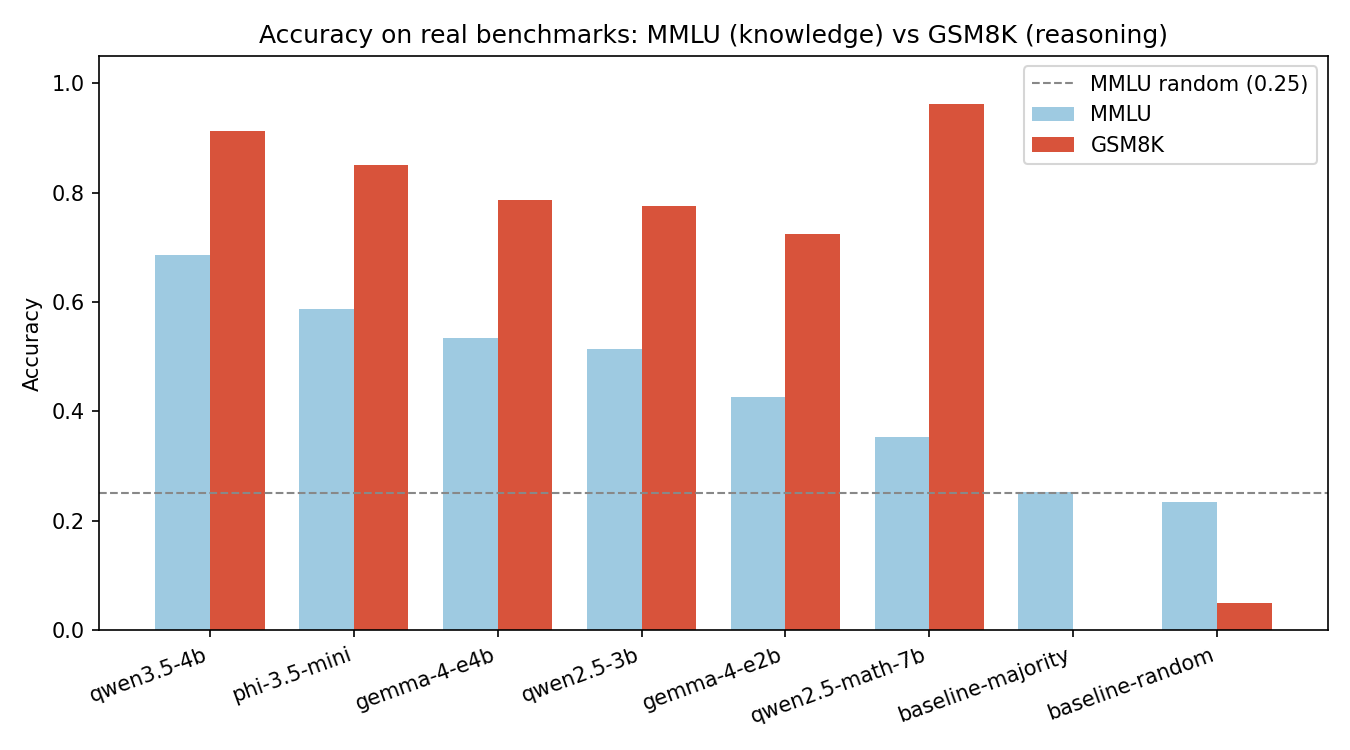
\includegraphics[width=0.8\linewidth]{images/saturation.png}
  \caption{Accuracy MMLU vs GSM8K theo model. GSM8K bám sát trần trên; MMLU trải
  rộng --- một benchmark còn ``đo được'', một benchmark đã ``bão hoà''.}
  \label{fig:saturation}
\end{figure}

\subsection{Rank-instability: chính benchmark chọn người thắng}

Đây là kết quả trung tâm. Bảng~\ref{tab:ranking} xếp hạng các model trên MMLU và
GSM8K \emph{riêng}. Trong panel năm model đa năng, thứ hạng trùng khít; nhưng
\textbf{math-specialist} làm thứ hạng \emph{rã}: nó đứng \textbf{hạng 1 GSM8K
(0.963)} nhưng \textbf{hạng 6 --- bét bảng --- trên MMLU (0.353)}, với
\texttt{rank\_shift} = 5.

\begin{table}[t]
\centering
\caption{Thứ hạng trên hai benchmark. Math-specialist lật từ hạng 6 (MMLU) lên
hạng 1 (GSM8K). Tương quan hạng Spearman $\rho = 0.14$ trên cả sáu model, và
$\rho = 0.0$ riêng nhóm $\geq 3$B.}
\label{tab:ranking}
\small
\begin{tabular}{lcccc}
\hline
\textbf{System} & \textbf{params\_b} & \textbf{rank\_mmlu} & \textbf{rank\_gsm8k} & \textbf{shift} \\
\hline
qwen3.5-4b      & 4.0 & 1 & 2 & 1 \\
phi-3.5-mini    & 3.8 & 2 & 3 & 1 \\
gemma-4-e4b     & 4.5 & 3 & 4 & 1 \\
qwen2.5-3b      & 3.1 & 4 & 5 & 1 \\
gemma-4-e2b     & 2.3 & 5 & 6 & 1 \\
qwen2.5-math-7b & 7.0 & \textbf{6} & \textbf{1} & \textbf{5} \\
\hline
\end{tabular}
\end{table}

Hệ quả định lượng: hệ số tương quan hạng \textbf{Spearman $\rho = 0.14$} cho cả sáu
model, và \textbf{$\rho = 0.0$} (không tương quan) cho riêng nhóm $\geq 3$B. Đáng
chú ý nhất: model \emph{to nhất panel} (7B) lại \emph{thua mọi model 2--4B trên
MMLU} trong khi \emph{thắng tất cả trên GSM8K}. Cần nói rõ phạm vi của kết luận này:
panel năm model đa năng \emph{vẫn} xếp hạng nhất quán giữa hai benchmark (chỉ shift
1 bậc, $\rho = 1.0$ nếu xét riêng); toàn bộ $\rho = 0.14$ là do \emph{một} model lệch
chủ đích (math-7b) gây ra. Vì vậy luận điểm không phải ``benchmark luôn đảo lộn mọi
thứ hạng'', mà là \textbf{một construct duy nhất đủ lệch so với panel là đủ để biến
``ai thắng'' thành \emph{hàm của việc chọn benchmark}} --- và đó chính là rủi ro mà
một bảng xếp hạng đơn-benchmark không bộc lộ. Hình~\ref{fig:agreement}
trực quan hoá: math-specialist nằm hẳn ngoài đám đông, ở góc dưới-phải (GSM8K cao,
MMLU thấp), phá vỡ đường chéo đồng thuận.

\begin{figure}[t]
  \centering
  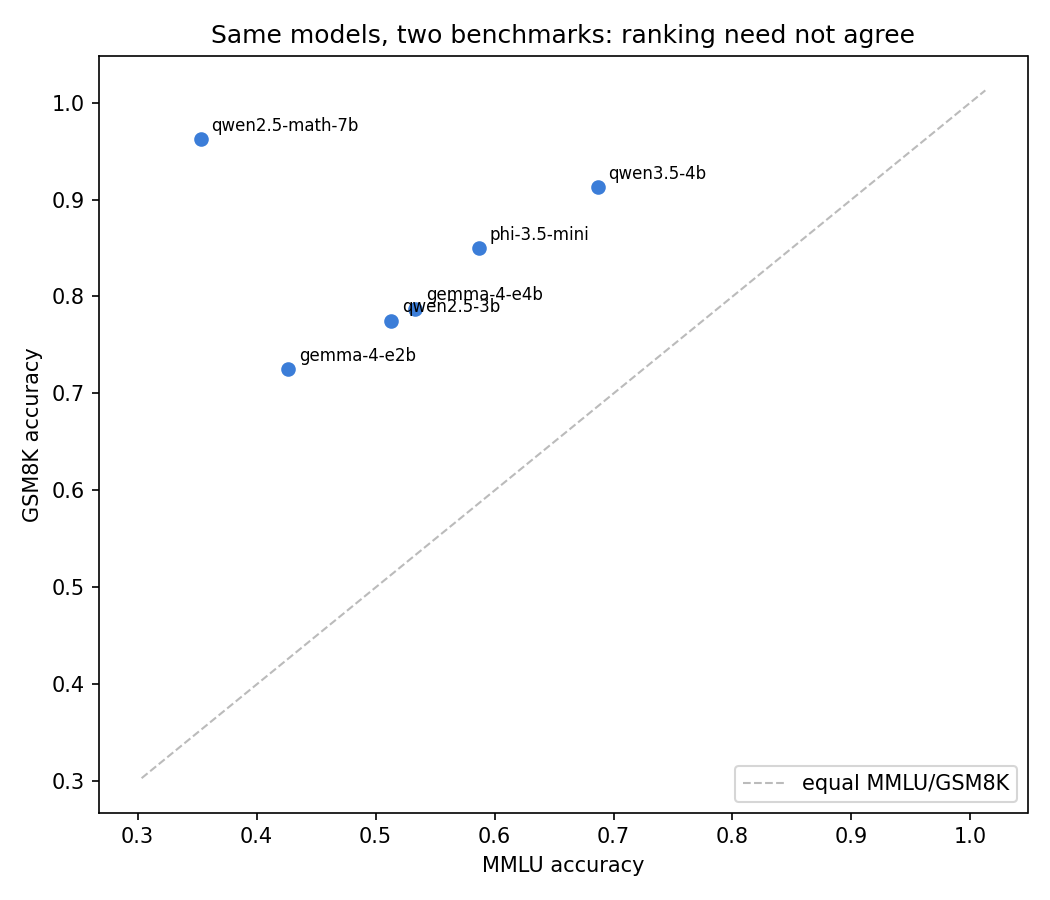
\includegraphics[width=0.7\linewidth]{images/model_agreement.png}
  \caption{Scatter MMLU $\times$ GSM8K. Năm model đa năng bám một đường đơn điệu;
  math-specialist (góc dưới-phải) phá thế đồng thuận $\Rightarrow$ thứ hạng phụ
  thuộc benchmark.}
  \label{fig:agreement}
\end{figure}

\paragraph{Minh bạch thiết kế.} Math-specialist là một \emph{đầu dò chủ đích lệch},
không thuộc panel $\sim$4B. Bản thân panel năm model đa năng xếp hạng \emph{trùng}
($\rho = 1.0$); chính việc \emph{thêm} một model lệch chuyên môn mới làm $\rho$ rã.
Nhóm khai báo rõ điều này: rank-instability là thứ phải \emph{đo}, và ở đây ta
\emph{dựng điều kiện để đo nó}, chứ không trình bày như hiện tượng tự nhiên xảy ra
ở mọi panel.

\subsection{Metric giòn: cùng câu trả lời, đổi cách chấm là sập điểm}

Bảng~\ref{tab:metricgap} cho thấy độ giòn của lớp chấm GSM8K. Với \emph{cùng một
đầu ra} của mô hình, bộ chấm \emph{naive} (lấy số đầu) cho accuracy $\approx 0$
trong khi bộ \emph{robust} (lấy số cuối) cho 0.73--0.96. Cột
\texttt{n\_robust\_only} --- số câu đúng bị bộ giòn đánh trượt --- lên tới
\textbf{58--77 trên 80 câu}.

\begin{table}[t]
\centering
\caption{GSM8K: hai bộ chấm khác nhau \emph{đúng một quyết định} (vị trí lấy số).
Chênh lệch khổng lồ $\Rightarrow$ \emph{metric $\neq$ construct}.}
\label{tab:metricgap}
\small
\begin{tabular}{lccc}
\hline
\textbf{System} & \textbf{acc\_naive} & \textbf{acc\_robust} & \textbf{n\_robust\_only} \\
\hline
qwen2.5-math-7b & 0.000 & 0.963 & 77 \\
qwen3.5-4b      & 0.013 & 0.913 & 72 \\
phi-3.5-mini    & 0.013 & 0.850 & 67 \\
gemma-4-e4b     & 0.000 & 0.788 & 63 \\
qwen2.5-3b      & 0.013 & 0.775 & 62 \\
gemma-4-e2b     & 0.000 & 0.725 & 58 \\
\hline
\end{tabular}
\end{table}

Đây là bằng chứng định lượng đậm nét cho luận điểm \emph{metric $\neq$ construct}:
năng lực thật của mô hình không đổi, nhưng một lựa chọn cài đặt tầm thường trong
lớp chấm có thể biến điểm từ 0.96 thành 0.00. Hình~\ref{fig:metricgap} minh hoạ
khoảng cách này; ví dụ cụ thể được phân tích ở Phần~\ref{sec:error}.

\begin{figure}[t]
  \centering
  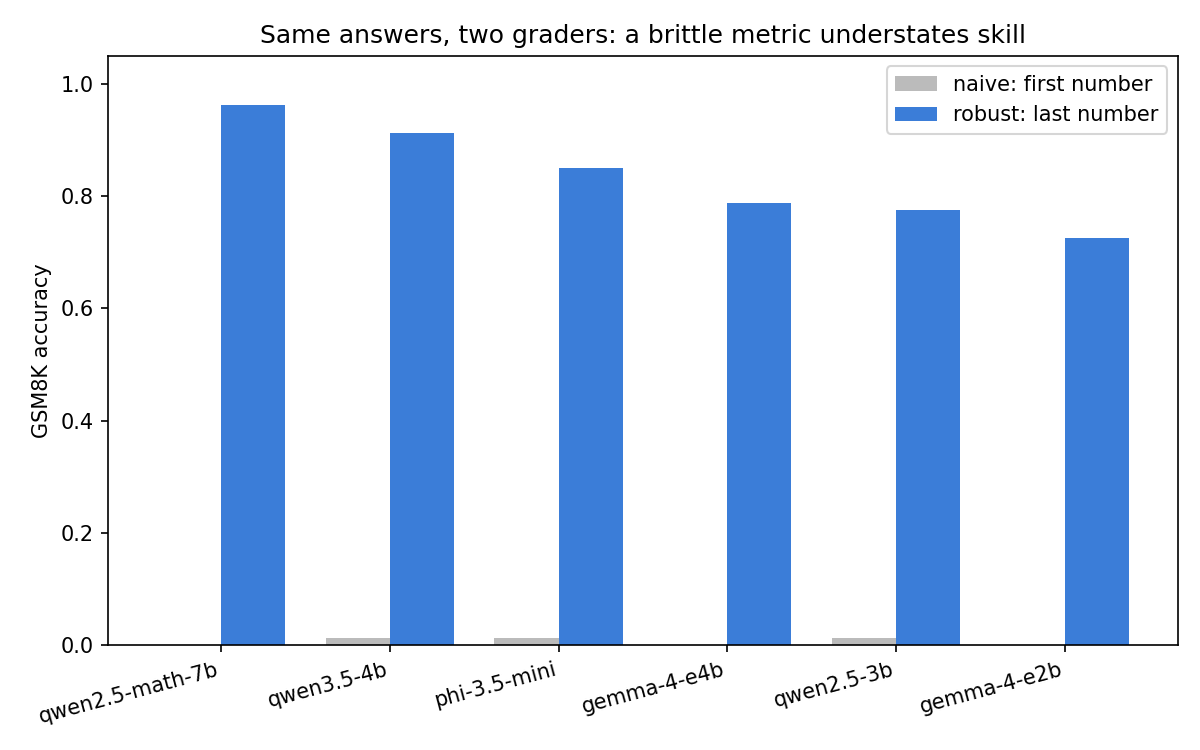
\includegraphics[width=0.8\linewidth]{images/metric_gap.png}
  \caption{GSM8K: accuracy theo bộ chấm \emph{naive} (số đầu) vs \emph{robust}
  (số cuối). Chỉ khác vị trí lấy số.}
  \label{fig:metricgap}
\end{figure}

\subsection{Phương sai construct: ``MMLU accuracy'' che giấu gì}

Hình~\ref{fig:subjects} (và \texttt{mmlu\_by\_subject.csv}) tách accuracy theo từng
môn MMLU. Cùng một model nhảy từ 0.0 ở vài môn (abstract\_algebra,
college\_mathematics) lên 1.0 ở môn khác (college\_computer\_science,
professional\_medicine). Một con số ``MMLU accuracy'' duy nhất do đó \emph{che
giấu} chênh lệch lớn giữa các môn $\Rightarrow$ ``MMLU'' không phải một construct
\emph{đồng nhất}. (Lưu ý: chỉ 2--5 câu/môn nên đây là minh hoạ định tính, không
phải ước lượng chắc theo từng môn.)

\begin{figure}[t]
  \centering
  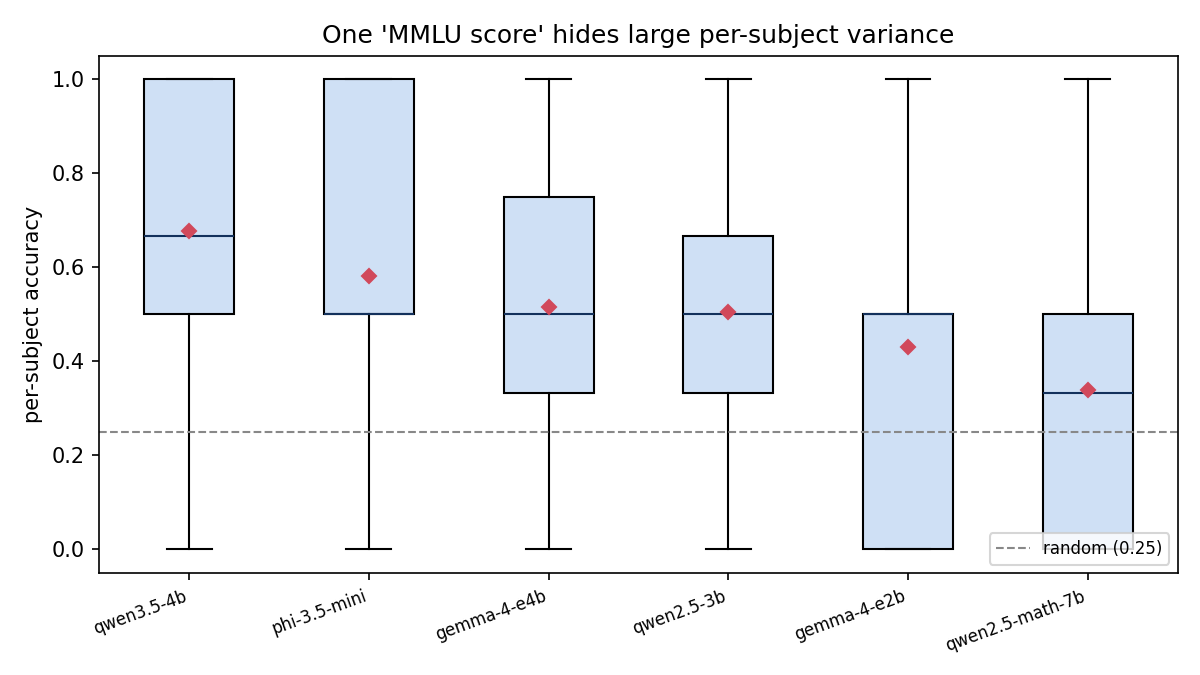
\includegraphics[width=0.85\linewidth]{images/mmlu_by_subject.png}
  \caption{Phân bố accuracy MMLU \emph{theo môn}, mỗi box ứng một model (kim cương
  đỏ = accuracy trung bình). Whisker trải gần như toàn dải $0$--$1$ cho thấy một
  con số ``MMLU accuracy'' duy nhất che giấu phương sai lớn giữa các môn $\Rightarrow$
  ``MMLU'' gộp nhiều construct khác nhau dưới một cái tên.}
  \label{fig:subjects}
\end{figure}

\subsection{Coverage: nhiễu đo lường lệch theo model}

\texttt{coverage.csv} ghi tỉ lệ câu \emph{trích được đáp án}. Trên GSM8K, coverage
= 1.0 cho mọi model; trên MMLU, coverage dao động \textbf{0.945--0.99} --- tức một
số model thi thoảng bị phạt vì \emph{không trích được đáp án} (lỗi format) chứ
không phải vì sai kiến thức. Đây là một nguồn nhiễu đo lường \emph{lệch theo model}
mà một bảng ``accuracy'' đơn thuần không bộc lộ.

\subsection{Robustness: điểm gốc dựa một phần vào format}

Bảng~\ref{tab:robust} (và Hình~\ref{fig:robust}) so accuracy gốc với accuracy trên
bản nhiễu giữ nhãn. Mọi model đều tụt \textbf{0.06--0.18}. Đáng chú ý, model
\emph{yếu MMLU nhất} (math-7b) tụt \emph{nhiều nhất} ($-0.18$): phần điểm MMLU của
nó dựa vào vị trí/format đáp án hơn là kiến thức thật --- đúng kiểu lỗ hổng mà
perturbation theo tinh thần SuperGLUE được thiết kế để phát hiện.

\begin{table}[t]
\centering
\caption{MMLU robustness: độ tụt accuracy khi đảo option / chèn distractor (giữ
nhãn). Tụt $> 0$ $\Rightarrow$ điểm gốc một phần dựa vào bề mặt câu hỏi.
\textbf{Lưu ý:} \texttt{acc\_original} ở đây tính trên \emph{đúng 50 câu được chọn
để perturbation}, nên khác accuracy toàn tập MMLU 150 câu ở Bảng~\ref{tab:accuracy}
(ví dụ math-7b: 0.46 trên tập con vs 0.353 toàn tập).}
\label{tab:robust}
\small
\begin{tabular}{lccc}
\hline
\textbf{System} & \textbf{acc\_original} & \textbf{acc\_perturbed} & \textbf{drop} \\
\hline
qwen2.5-math-7b & 0.46 & 0.28 & 0.18 \\
qwen3.5-4b      & 0.66 & 0.50 & 0.16 \\
qwen2.5-3b      & 0.56 & 0.46 & 0.10 \\
gemma-4-e4b     & 0.52 & 0.42 & 0.10 \\
phi-3.5-mini    & 0.58 & 0.50 & 0.08 \\
gemma-4-e2b     & 0.44 & 0.38 & 0.06 \\
\hline
\end{tabular}
\end{table}

\begin{figure}[t]
  \centering
  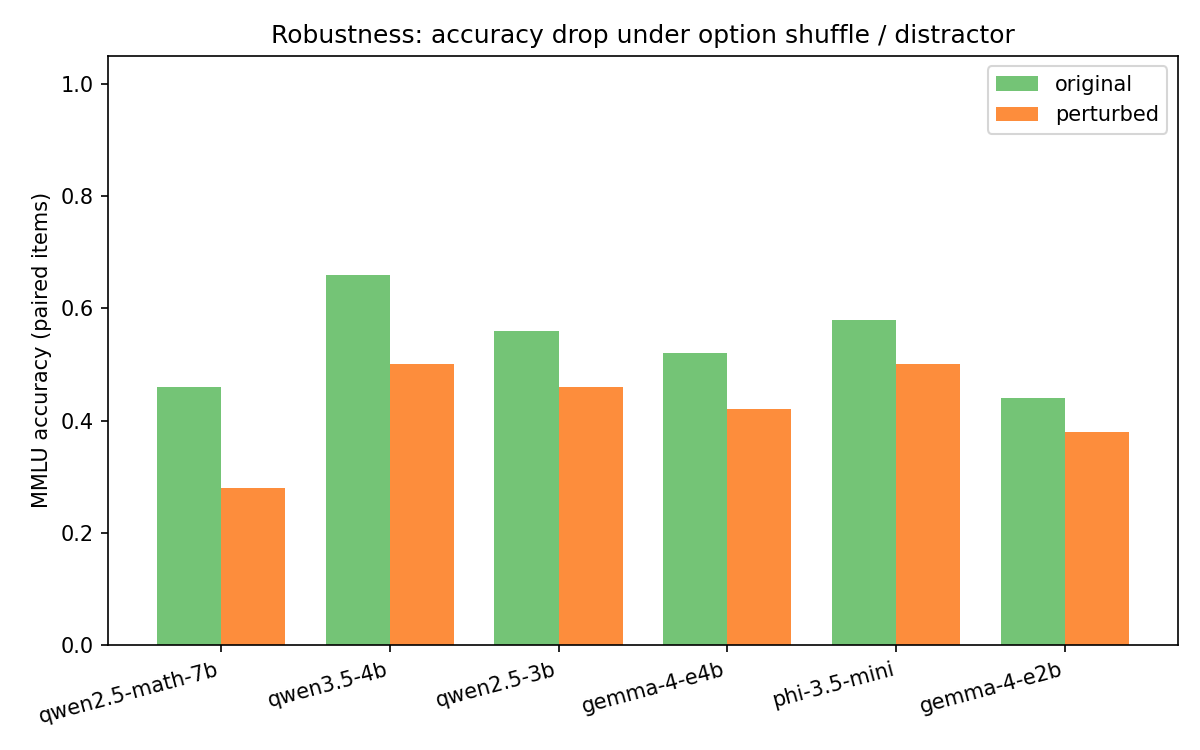
\includegraphics[width=0.8\linewidth]{images/robustness.png}
  \caption{MMLU: accuracy gốc vs accuracy sau nhiễu giữ nhãn. Mọi model đều tụt.}
  \label{fig:robust}
\end{figure}

\subsection{Cảnh báo nhiễm dữ liệu}

Một quan sát phải nêu thẳng: cả MMLU (2021) và GSM8K (2021) gần như chắc nằm trong
dữ liệu huấn luyện của các model này. Việc \textbf{GSM8K đạt $\sim$0.9 cho model
chỉ 3--4B} nhiều khả năng phản ánh \emph{trí nhớ/nhiễm dữ liệu} hơn là \emph{suy
luận} thuần. Vì vậy các điểm tuyệt đối \emph{không} nên đọc như ``năng lực thật'';
demo dùng chúng để \emph{phơi bày chính vấn đề này}, không để xếp hạng. (Robustness
tụt vừa phải cho thấy mô hình không bám chuỗi test verbatim, nhưng không loại trừ
nhiễm ở mức ngữ nghĩa.)

\section{Kết quả định tính, phân tích lỗi và nhận xét từ demo}
\label{sec:error}

Bên cạnh các con số, demo xuất hai tệp định tính: \texttt{error\_analysis.csv}
(mọi câu sai, kèm đầu ra thô) và \texttt{metric\_gap\_examples.csv} (các câu mô
hình \emph{đúng} nhưng bộ chấm giòn đánh trượt). Phần này phân tích các \emph{kiểu
lỗi} và rút ra nhận xét.

\subsection{Lỗi của \emph{phép đo}, không phải của mô hình}

Đáng chú ý nhất là loại ``lỗi'' \emph{không phải} của mô hình mà của \emph{cách
chấm}. Xét câu \texttt{gsm8k\_0000} (đáp án đúng = 100). Mô hình suy luận:

\begin{quote}\small\itshape
``\ldots Trường chi trả một nửa tổng chi phí. Phần trường trả $= \$300 \times
\tfrac{1}{2} = \$150$\ldots'' $\Rightarrow$ \ldots $\Rightarrow$ đáp số cuối $= 100$.
\end{quote}

Bộ chấm \emph{robust} lấy số \emph{cuối} ($100$) $\Rightarrow$ \textbf{đúng}. Bộ
chấm \emph{naive} lấy số \emph{đầu} (\$300 hoặc \$150 --- một số trung gian)
$\Rightarrow$ \textbf{sai}. Mô hình không hề sai; lớp \texttt{re.search(r"\textbackslash
d+")} ngây thơ mới sai. Trên toàn tập, kiểu này chiếm \textbf{58--77/80 câu} mỗi
model (Bảng~\ref{tab:metricgap}). Bài học: với benchmark đầu ra dài, \emph{lớp trích
xuất/chấm} là chỗ dễ hỏng nhất --- đúng lý do SWE-bench chọn chấm bằng \emph{thực
thi test} thay vì so chuỗi.

\subsection{Lỗi format vs lỗi kiến thức (coverage)}

Một số câu MMLU ``sai'' thực ra là \emph{không trích được đáp án}: mô hình diễn giải
dài dòng, lảng tránh, hoặc không nêu rõ một chữ cái \texttt{A/B/C/D}. Coverage MMLU
0.945--0.99 cho thấy 1--5\% câu rơi vào loại này tuỳ model. Gộp chung loại lỗi
format với loại sai kiến thức vào một con số ``accuracy'' sẽ \emph{trộn} hai nguồn
sai có bản chất khác nhau --- và nhiễu này \emph{lệch theo model}.

\subsection{Lỗi do nhiễu bề mặt (robustness)}

Trên bản nhiễu giữ nhãn, một số câu mô hình \emph{đúng ở bản gốc} lại \emph{sai} chỉ
vì đảo vị trí đáp án hoặc thêm ``None of the above''. Vì nhãn không đổi, đây là bằng
chứng mô hình \emph{một phần} dựa vào vị trí/format thay vì nội dung. Độ tụt
0.06--0.18 (Bảng~\ref{tab:robust}) lượng hoá phần ``điểm ăn may theo bề mặt'' đó.

\subsection{Nhận xét tổng hợp từ demo}

\begin{enumerate}
  \item \textbf{Điểm số là \emph{có ý nghĩa} nhưng \emph{không tuyệt đối}}: mọi
    model vượt xa baseline (có tín hiệu thật), nhưng nhiễm dữ liệu khiến điểm GSM8K
    không nên đọc như năng lực suy luận thuần.
  \item \textbf{Không một benchmark nào xếp hạng được model}: $\rho = 0.14$
    (toàn bộ) và $\rho = 0.0$ ($\geq 3$B) cho thấy thứ hạng phụ thuộc \emph{lựa
    chọn benchmark}; model to nhất vẫn có thể bét bảng ở một construct.
  \item \textbf{Metric $\neq$ construct}: một quyết định cài đặt nhỏ trong lớp chấm
    đổi điểm từ 0.96 xuống 0.00 --- benchmark dễ sai ở \emph{cách chấm} hơn ở
    \emph{câu hỏi}.
  \item \textbf{``MMLU accuracy'' là một số gộp}: phương sai theo môn rất lớn nên
    một con số tổng che giấu việc đo nhiều construct khác nhau.
  \item \textbf{Đo lường luôn có nhiễu lệch}: coverage và robustness cho thấy điểm
    bị nhiễu bởi format và bề mặt, và nhiễu này khác nhau giữa các model.
\end{enumerate}

Tất cả các nhận xét trên đều khớp với khung \emph{construct validity}
(\cite{measuring_what_matters}) và bộ tiêu chí \emph{BetterBench}
(\cite{betterbench}): một demo nhỏ, khi soi đúng chỗ, đủ để cho thấy
\emph{bản thân phép đo} mới là đối tượng cần được đánh giá --- đúng thông điệp
``What's Measured, What's Missing, What's Next'' của tutorial.

\section{Hướng dẫn tái lập demo}
\label{sec:repro}

Demo được thiết kế để \emph{bất kỳ ai cũng chạy lại được}, đúng tiêu chí
\emph{reproducibility} của BetterBench~\cite{betterbench}. Có ba cơ chế
bảo đảm tính tất định.

\subsection{Ba trụ cột tái lập}

\begin{enumerate}
  \item \textbf{Dữ liệu cố định theo seed}: tập con benchmark lấy bằng
    \texttt{SEED = 0} và ghi ra \texttt{data/*.jsonl} $\Rightarrow$ mọi người nhận
    \emph{đúng cùng item, cùng thứ tự}.
  \item \textbf{Sinh văn bản greedy}: \texttt{do\_sample=False} $\Rightarrow$ đầu
    ra không phụ thuộc ngẫu nhiên; chạy lại cho đúng cùng văn bản.
  \item \textbf{Cache theo nội dung}: mỗi lời gọi lưu theo
    \texttt{sha256(model\_id, prompt)} trong \texttt{results/predictions/}. Cache
    lưu văn bản thô, điểm \emph{tính lại} mỗi lần $\Rightarrow$ tái sinh toàn bộ
    bảng/biểu đồ \emph{không cần GPU}, và thêm model mới chỉ tốn chi phí cho phần
    mới.
\end{enumerate}

\subsection{Cách A --- Kaggle}

\begin{enumerate}
  \item Mở \texttt{notebook/2\_run\_all.ipynb}. Settings $\to$ Accelerator
    $\to$ \texttt{GPU T4}; Internet $\to$ On.
  \item Add-ons $\to$ Secrets $\to$ thêm \texttt{HF\_TOKEN} (HF read token). Chấp
    nhận licence Gemma trên Hugging Face (các model khác ungated).
  \item \emph{Run all}. Vì greedy + cache, bấm lại ra \emph{đúng cùng số}. Lần đầu
    $\sim$1.5--2 giờ; các lần sau gần như tức thì.
\end{enumerate}

\subsection{Cách B --- Máy có GPU NVIDIA $\geq 8$GB}

\begin{verbatim}
python -m venv .venv && source .venv/bin/activate
pip install -r requirements.txt
huggingface-cli login          # cần đã accept licence Gemma
python src/evaluate.py         # -> results/per_item.csv
python src/analysis.py         # -> results/*.csv + images/*.png
\end{verbatim}

\subsection{Cách C --- Không có GPU (chỉ kiểm tra pipeline)}

\begin{verbatim}
pip install pandas matplotlib numpy
MINIBENCH_SYNTHETIC=1 python src/evaluate.py --fake
MINIBENCH_SYNTHETIC=1 python src/analysis.py
\end{verbatim}

Đường này dùng \texttt{FakeRunner} + dữ liệu tổng hợp để chứng minh \emph{toàn bộ
luồng} chạy được trên máy không GPU; \textbf{số liệu sinh ra không dùng để báo cáo}
--- chỉ để kiểm tra code.

\subsection{Sản phẩm tái lập}

Sau khi chạy, \texttt{results/} chứa: \texttt{per\_item.csv} (từng câu),
\texttt{accuracy.csv}, \texttt{ranking.csv}, \texttt{coverage.csv},
\texttt{mmlu\_by\_subject.csv}, \texttt{metric\_gap.csv} (+\texttt{\_examples}),
\texttt{robustness.csv}, \texttt{error\_analysis.csv}, và \texttt{images/*.png}.
Mã nguồn và cache prediction được công khai trong repo, nên kết quả trong báo cáo
này có thể được \emph{tái kiểm} đầy đủ.

\subsection{Giới hạn của tái lập}

Tái lập \emph{tất định} chỉ đúng với cùng phiên bản thư viện (\texttt{transformers},
\texttt{bitsandbytes}) và cùng phần cứng; lượng tử hoá 4-bit và kernel GPU khác nhau
có thể gây sai khác nhỏ ở biên. Tuy nhiên cơ chế cache văn bản thô giúp các \emph{con
số trong báo cáo} luôn tái sinh được từ chính các prediction đã lưu, độc lập với
phần cứng.


\Needspace{10\baselineskip}

\small
\setlength{\tabcolsep}{6pt}
\renewcommand{\arraystretch}{1.2}

\begin{longtable}{p{2.2cm} p{3.6cm} p{10.2cm}}
\caption{Phân công công việc và mức độ hoàn thành của các thành viên trong tutorial “The Science of Benchmarking”.}
\label{tab:work_distribution_benchmarking} \\

\toprule
\textbf{MSSV} & \textbf{Họ và tên} & \textbf{Phần đóng góp} \\
\midrule
\endfirsthead

\toprule
\textbf{MSSV} & \textbf{Họ và tên} & \textbf{Phần đóng góp} \\
\midrule
\endhead

23120048 & Phan Hoàng Quốc Huy &
\textbf{Nền tảng benchmarking và “What’s Measured”.}
Phụ trách giới thiệu tổng quan, bối cảnh AI/ML benchmarking, các khái niệm nền (metric, dataset, evaluation protocol, construct validity, data contamination, Goodhart’s Law…).
Viết các mục 01--05 của báo cáo (\texttt{01\_introduction.tex} -- \texttt{05\_whats\_measured.tex}); thiết kế slide 1--12.
Paper chính: \emph{AI and the Everything in the Whole Wide World Benchmark}, \emph{Measuring what Matters}.
Hoàn thành 100\% nội dung nền tảng và Q\&A. \\
\addlinespace

23120030 & Trần Thanh Đạt &
\textbf{Chất lượng benchmark và case study truyền thống.}
Trình bày tiêu chí benchmark tốt, khung BetterBench để đánh giá chất lượng benchmark, phân tích case study GLUE (benchmark suite NLU cổ điển).
Viết các mục 06--08 (\texttt{06\_benchmark\_quality.tex} -- \texttt{08\_glue.tex}); slide 13--18.
Paper chính: \emph{BetterBench}, \emph{GLUE}.
Hoàn thành 100\% phần đánh giá benchmark và GLUE. \\
\addlinespace

23122006 & Lưu Thượng Hồng &
\textbf{SuperGLUE và “What’s Missing”.}
Phân tích hiện tượng bão hòa benchmark (saturation, ceiling effect), lý do ra đời SuperGLUE, tổng hợp những hạn chế còn thiếu của benchmark hiện tại (data, measurement, systemic, epistemic issues).
Viết các mục 09--11 (\texttt{09\_superglue.tex} -- \texttt{11\_discussion.tex}); slide 19--24.
Paper chính: \emph{SuperGLUE}, kết hợp \emph{BetterBench}.
Hoàn thành 100\% phần SuperGLUE và nhận diện các vấn đề chưa được giải quyết. \\
\addlinespace

23120041 & Lê Minh Hải &
\textbf{Benchmark thế hệ mới và SWE-bench.}
Giới thiệu xu hướng real‑world và agentic benchmark; phân tích case study SWE-bench (đánh giá mô hình ngôn ngữ trên GitHub issues thực tế).
Thiết kế cấu trúc demo đa tác vụ mô phỏng ý tưởng từ GLUE, SuperGLUE và SWE-bench.
Viết mục 12--13 (\texttt{12\_whats\_next.tex}, \texttt{13\_swe\_bench.tex}) và phần mô tả tổng quan demo trong mục 14; slide 25--28.
Hoàn thành 100\% nội dung “What’s Next” và kiến trúc demo. \\
\addlinespace

23120088 & Cao Tiến Thành &
\textbf{Thực nghiệm, kết quả và hoàn thiện sản phẩm.}
Xây dựng dataset nhỏ cho demo, cài đặt metric (accuracy, exact match, pass/fail, robustness), viết mã nguồn (\texttt{run\_evaluation.py}, \texttt{metrics.py}, \texttt{visualize.py}), chạy thực nghiệm trên ít nhất hai model/prompt.
Viết các mục 14--20 (\texttt{14\_demo\_design.tex} -- \texttt{20\_reproducibility.tex}); slide 29--34; soạn README, \texttt{requirements.txt}, đóng gói toàn bộ thư mục demo và kiểm tra khả năng tái lập.
Hoàn thành 100\% demo, kết quả định lượng/định tính, biểu đồ và tài liệu hướng dẫn. \\
\bottomrule

\end{longtable}

% ============ TÀI LIỆU THAM KHẢO ============
\input{ref/ref.tex}

\end{document}